% Options for packages loaded elsewhere
\PassOptionsToPackage{unicode}{hyperref}
\PassOptionsToPackage{hyphens}{url}
%
\documentclass[
]{book}
\usepackage{amsmath,amssymb}
\usepackage{lmodern}
\usepackage{iftex}
\ifPDFTeX
  \usepackage[T1]{fontenc}
  \usepackage[utf8]{inputenc}
  \usepackage{textcomp} % provide euro and other symbols
\else % if luatex or xetex
  \usepackage{unicode-math}
  \defaultfontfeatures{Scale=MatchLowercase}
  \defaultfontfeatures[\rmfamily]{Ligatures=TeX,Scale=1}
\fi
% Use upquote if available, for straight quotes in verbatim environments
\IfFileExists{upquote.sty}{\usepackage{upquote}}{}
\IfFileExists{microtype.sty}{% use microtype if available
  \usepackage[]{microtype}
  \UseMicrotypeSet[protrusion]{basicmath} % disable protrusion for tt fonts
}{}
\makeatletter
\@ifundefined{KOMAClassName}{% if non-KOMA class
  \IfFileExists{parskip.sty}{%
    \usepackage{parskip}
  }{% else
    \setlength{\parindent}{0pt}
    \setlength{\parskip}{6pt plus 2pt minus 1pt}}
}{% if KOMA class
  \KOMAoptions{parskip=half}}
\makeatother
\usepackage{xcolor}
\IfFileExists{xurl.sty}{\usepackage{xurl}}{} % add URL line breaks if available
\IfFileExists{bookmark.sty}{\usepackage{bookmark}}{\usepackage{hyperref}}
\hypersetup{
  pdftitle={Introducción a R y Tidyverse},
  pdfauthor={Healthinnovation},
  hidelinks,
  pdfcreator={LaTeX via pandoc}}
\urlstyle{same} % disable monospaced font for URLs
\usepackage{color}
\usepackage{fancyvrb}
\newcommand{\VerbBar}{|}
\newcommand{\VERB}{\Verb[commandchars=\\\{\}]}
\DefineVerbatimEnvironment{Highlighting}{Verbatim}{commandchars=\\\{\}}
% Add ',fontsize=\small' for more characters per line
\usepackage{framed}
\definecolor{shadecolor}{RGB}{248,248,248}
\newenvironment{Shaded}{\begin{snugshade}}{\end{snugshade}}
\newcommand{\AlertTok}[1]{\textcolor[rgb]{0.94,0.16,0.16}{#1}}
\newcommand{\AnnotationTok}[1]{\textcolor[rgb]{0.56,0.35,0.01}{\textbf{\textit{#1}}}}
\newcommand{\AttributeTok}[1]{\textcolor[rgb]{0.77,0.63,0.00}{#1}}
\newcommand{\BaseNTok}[1]{\textcolor[rgb]{0.00,0.00,0.81}{#1}}
\newcommand{\BuiltInTok}[1]{#1}
\newcommand{\CharTok}[1]{\textcolor[rgb]{0.31,0.60,0.02}{#1}}
\newcommand{\CommentTok}[1]{\textcolor[rgb]{0.56,0.35,0.01}{\textit{#1}}}
\newcommand{\CommentVarTok}[1]{\textcolor[rgb]{0.56,0.35,0.01}{\textbf{\textit{#1}}}}
\newcommand{\ConstantTok}[1]{\textcolor[rgb]{0.00,0.00,0.00}{#1}}
\newcommand{\ControlFlowTok}[1]{\textcolor[rgb]{0.13,0.29,0.53}{\textbf{#1}}}
\newcommand{\DataTypeTok}[1]{\textcolor[rgb]{0.13,0.29,0.53}{#1}}
\newcommand{\DecValTok}[1]{\textcolor[rgb]{0.00,0.00,0.81}{#1}}
\newcommand{\DocumentationTok}[1]{\textcolor[rgb]{0.56,0.35,0.01}{\textbf{\textit{#1}}}}
\newcommand{\ErrorTok}[1]{\textcolor[rgb]{0.64,0.00,0.00}{\textbf{#1}}}
\newcommand{\ExtensionTok}[1]{#1}
\newcommand{\FloatTok}[1]{\textcolor[rgb]{0.00,0.00,0.81}{#1}}
\newcommand{\FunctionTok}[1]{\textcolor[rgb]{0.00,0.00,0.00}{#1}}
\newcommand{\ImportTok}[1]{#1}
\newcommand{\InformationTok}[1]{\textcolor[rgb]{0.56,0.35,0.01}{\textbf{\textit{#1}}}}
\newcommand{\KeywordTok}[1]{\textcolor[rgb]{0.13,0.29,0.53}{\textbf{#1}}}
\newcommand{\NormalTok}[1]{#1}
\newcommand{\OperatorTok}[1]{\textcolor[rgb]{0.81,0.36,0.00}{\textbf{#1}}}
\newcommand{\OtherTok}[1]{\textcolor[rgb]{0.56,0.35,0.01}{#1}}
\newcommand{\PreprocessorTok}[1]{\textcolor[rgb]{0.56,0.35,0.01}{\textit{#1}}}
\newcommand{\RegionMarkerTok}[1]{#1}
\newcommand{\SpecialCharTok}[1]{\textcolor[rgb]{0.00,0.00,0.00}{#1}}
\newcommand{\SpecialStringTok}[1]{\textcolor[rgb]{0.31,0.60,0.02}{#1}}
\newcommand{\StringTok}[1]{\textcolor[rgb]{0.31,0.60,0.02}{#1}}
\newcommand{\VariableTok}[1]{\textcolor[rgb]{0.00,0.00,0.00}{#1}}
\newcommand{\VerbatimStringTok}[1]{\textcolor[rgb]{0.31,0.60,0.02}{#1}}
\newcommand{\WarningTok}[1]{\textcolor[rgb]{0.56,0.35,0.01}{\textbf{\textit{#1}}}}
\usepackage{longtable,booktabs,array}
\usepackage{calc} % for calculating minipage widths
% Correct order of tables after \paragraph or \subparagraph
\usepackage{etoolbox}
\makeatletter
\patchcmd\longtable{\par}{\if@noskipsec\mbox{}\fi\par}{}{}
\makeatother
% Allow footnotes in longtable head/foot
\IfFileExists{footnotehyper.sty}{\usepackage{footnotehyper}}{\usepackage{footnote}}
\makesavenoteenv{longtable}
\usepackage{graphicx}
\makeatletter
\def\maxwidth{\ifdim\Gin@nat@width>\linewidth\linewidth\else\Gin@nat@width\fi}
\def\maxheight{\ifdim\Gin@nat@height>\textheight\textheight\else\Gin@nat@height\fi}
\makeatother
% Scale images if necessary, so that they will not overflow the page
% margins by default, and it is still possible to overwrite the defaults
% using explicit options in \includegraphics[width, height, ...]{}
\setkeys{Gin}{width=\maxwidth,height=\maxheight,keepaspectratio}
% Set default figure placement to htbp
\makeatletter
\def\fps@figure{htbp}
\makeatother
\setlength{\emergencystretch}{3em} % prevent overfull lines
\providecommand{\tightlist}{%
  \setlength{\itemsep}{0pt}\setlength{\parskip}{0pt}}
\setcounter{secnumdepth}{5}
\usepackage{booktabs}
\ifLuaTeX
  \usepackage{selnolig}  % disable illegal ligatures
\fi
\usepackage[]{natbib}
\bibliographystyle{plainnat}

\title{Introducción a R y Tidyverse}
\author{Healthinnovation}
\date{2022-05-26}

\begin{document}
\maketitle

{
\setcounter{tocdepth}{1}
\tableofcontents
}
\hypertarget{bienvenidos}{%
\chapter{¡Bienvenidos!}\label{bienvenidos}}

\hypertarget{acerca-del-curso}{%
\section{Acerca del curso}\label{acerca-del-curso}}

\hypertarget{exploraciuxf3n-competencial}{%
\section{Exploración competencial}\label{exploraciuxf3n-competencial}}

\hypertarget{sesiuxf3n-01}{%
\chapter{Sesión 01}\label{sesiuxf3n-01}}

\hypertarget{quuxe9-es-ciencia-de-datos}{%
\subsection{¿Qué es Ciencia de Datos?}\label{quuxe9-es-ciencia-de-datos}}

La Ciencia de Datos es una fusión entre múltiples disciplinas, incluyendo matematicas, estadistica, informatica, y tecnologia de la información.

La Ciencia de Datos permite extraer información relevante de los datos.

\begin{center}\includegraphics[width=0.6\linewidth]{https://healthinnovation.github.io/curso-introduccion-r-tidyverse/sesion_01/img/ciencia_datos_1} \end{center}

\hypertarget{por-quuxe9-usar-r-para-ciencia-de-datos}{%
\subsection{¿Por qué usar R para Ciencia de Datos?}\label{por-quuxe9-usar-r-para-ciencia-de-datos}}

R cuenta con las herramientas necesarias (entorno, librerías, y funciones) para desarrollar proyectos de Ciencia de Datos.

\begin{center}\includegraphics[width=0.9\linewidth]{https://user-images.githubusercontent.com/23284899/164085004-8f34ca37-3780-4790-91cc-c934f594b34b} \end{center}

\hypertarget{reconocimiento-rstudio}{%
\subsection{Reconocimiento Rstudio}\label{reconocimiento-rstudio}}

\begin{center}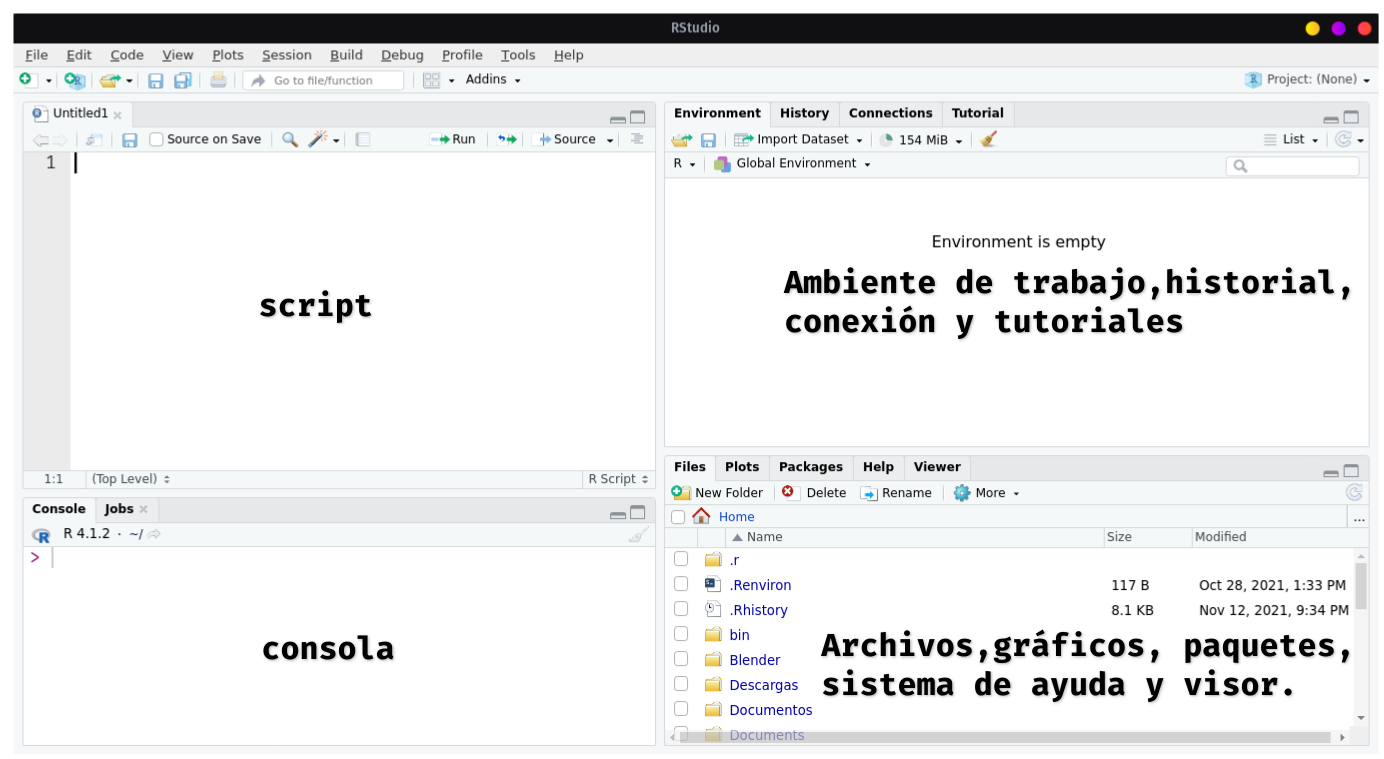
\includegraphics[width=0.85\linewidth]{https://healthinnovation.github.io/curso-introduccion-r-tidyverse/sesion_01/img/01_IDE_Rdtudio_v1} \end{center}

\begin{center}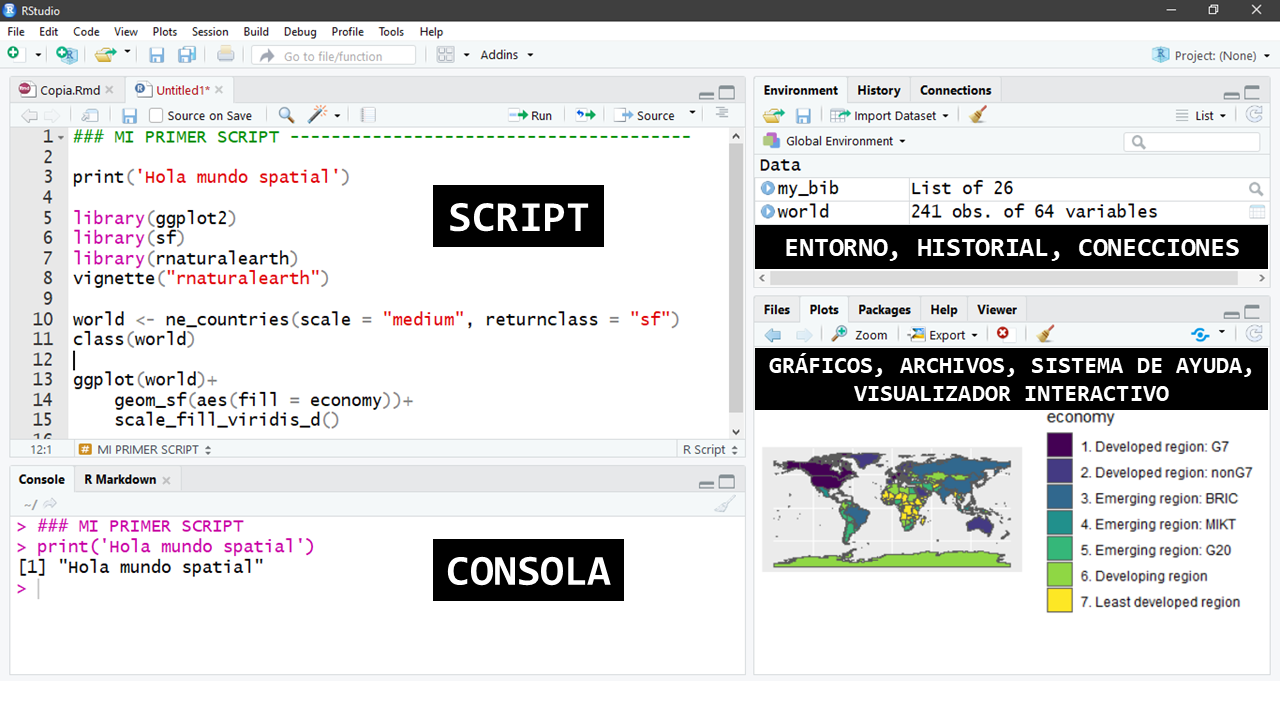
\includegraphics[width=0.85\linewidth]{https://healthinnovation.github.io/curso-introduccion-r-tidyverse/sesion_01/img/01_IDE_Rdtudio_v2} \end{center}

\hypertarget{mover-paneles}{%
\subsection{Mover paneles}\label{mover-paneles}}

\begin{center}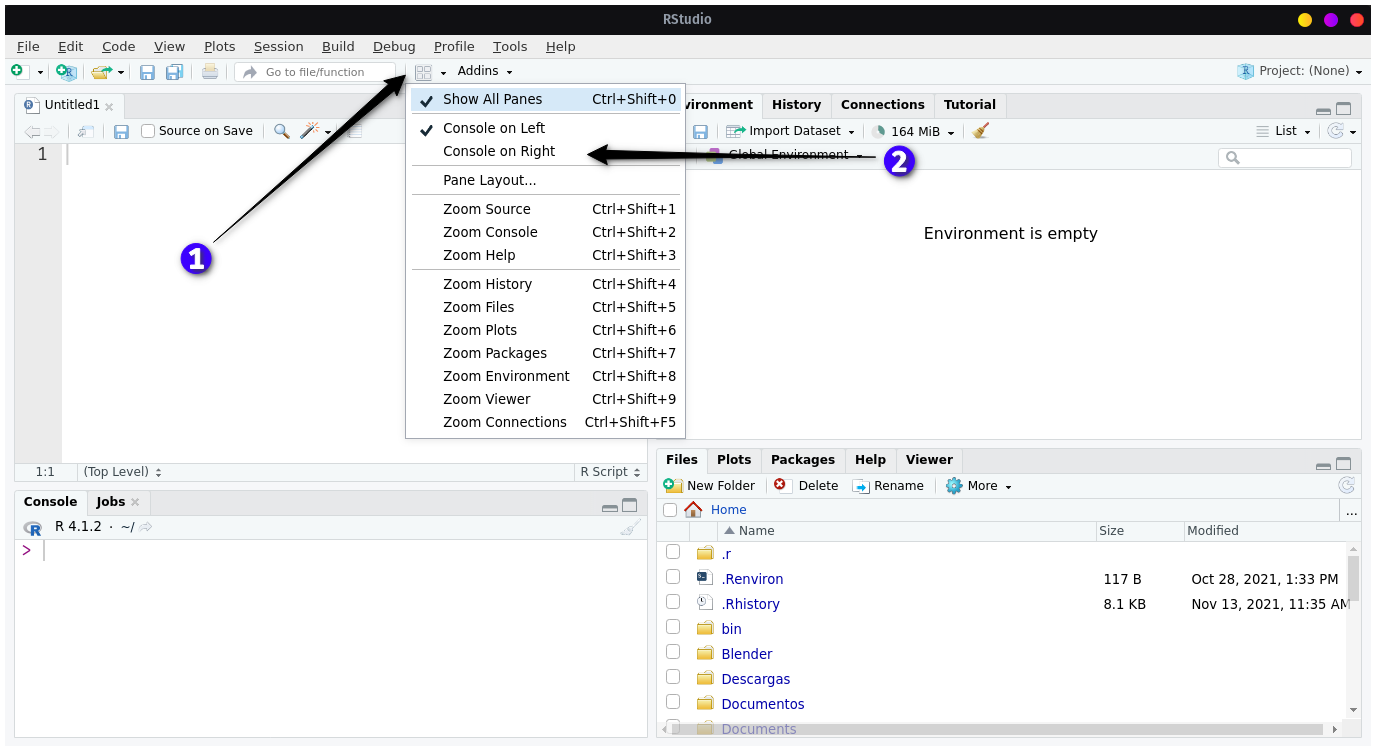
\includegraphics[width=0.85\linewidth]{https://healthinnovation.github.io/curso-introduccion-r-tidyverse/sesion_01/img/03_panel_v1} \end{center}

\begin{center}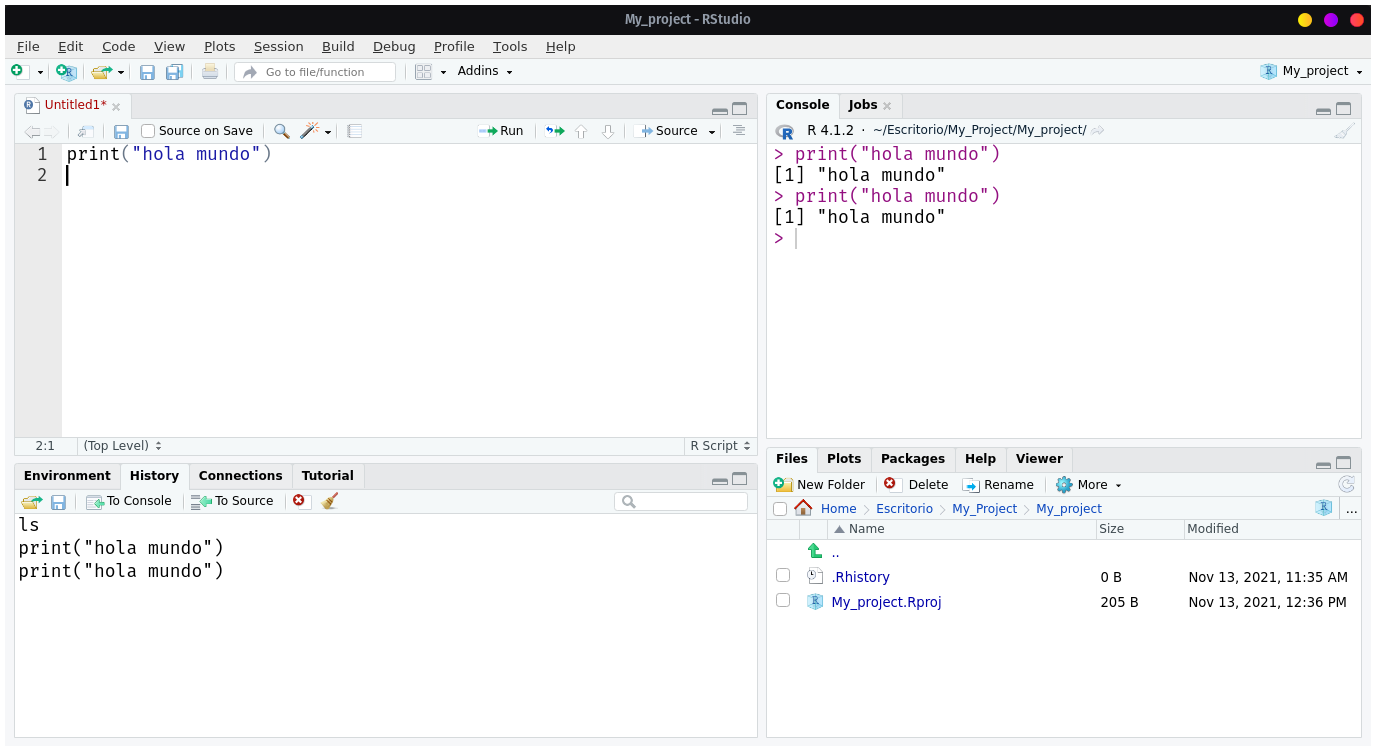
\includegraphics[width=0.85\linewidth]{https://healthinnovation.github.io/curso-introduccion-r-tidyverse/sesion_01/img/03_panel_v2} \end{center}

\hypertarget{personalizaciuxf3n-de-rstudio}{%
\subsection{Personalización de Rstudio}\label{personalizaciuxf3n-de-rstudio}}

\begin{center}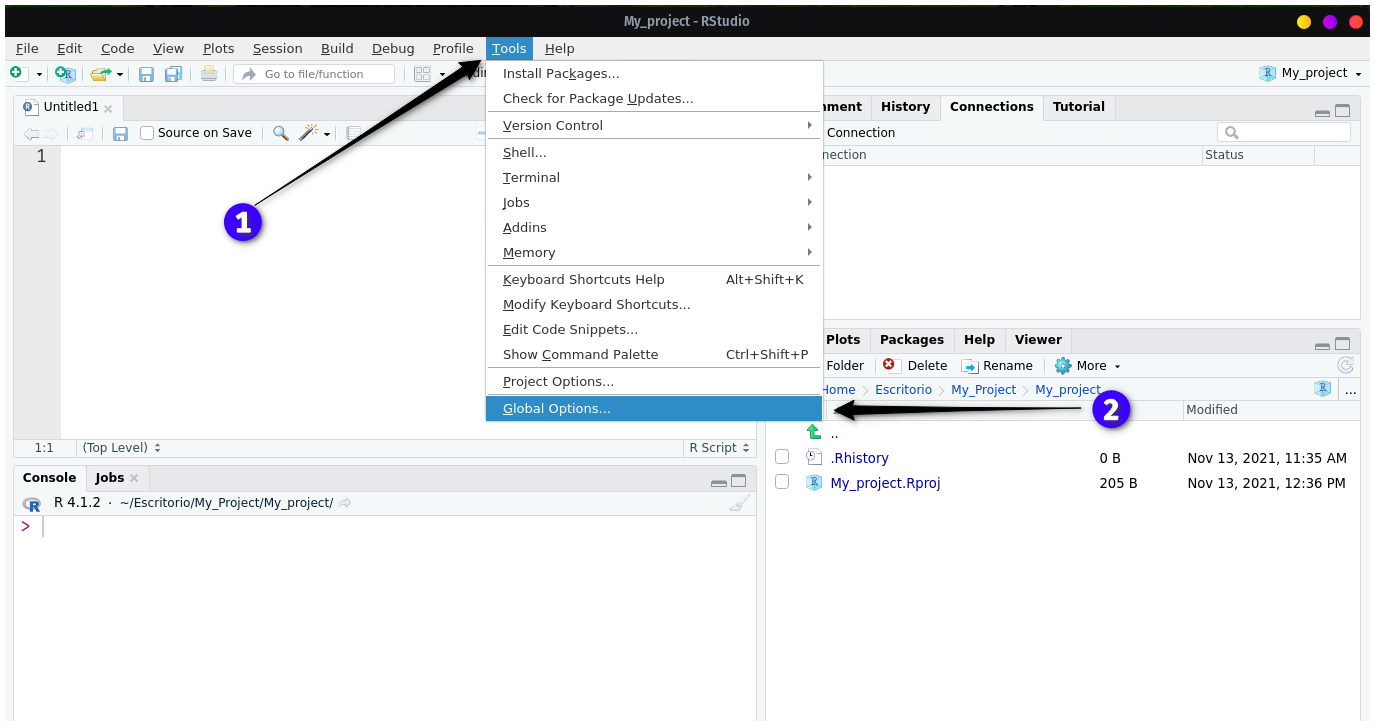
\includegraphics[width=0.85\linewidth]{https://healthinnovation.github.io/curso-introduccion-r-tidyverse/sesion_01/img/04_config_global_v1} \end{center}

\hypertarget{modificaciones-sobre-la-interfaz-de-rstudio}{%
\subsubsection{\texorpdfstring{\textbf{Modificaciones sobre la interfaz de Rstudio:}}{Modificaciones sobre la interfaz de Rstudio:}}\label{modificaciones-sobre-la-interfaz-de-rstudio}}

\begin{itemize}
\item
  Aumentar el zoom o utilizar el atajo: Ctrl y +
\item
  Cambiar tipo de letra puede hacer un tanto más agradable la codificación. La letra Fira
\item
  Code es bastante recomendable, pero se requiere instalar.
\item
  El tema también puede ayudar en que la codificación sea más agradable. El paquete rsthemes, contiene muchos temas extras.
\end{itemize}

\begin{center}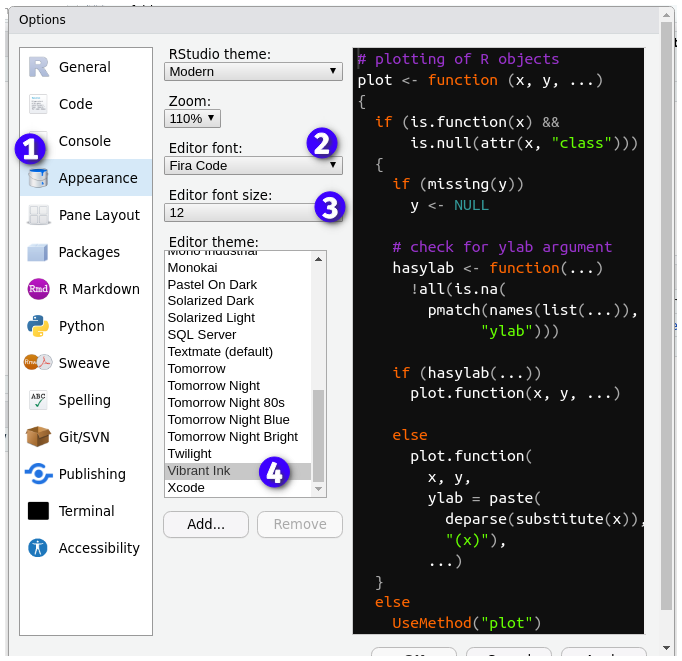
\includegraphics[width=0.85\linewidth]{https://healthinnovation.github.io/curso-introduccion-r-tidyverse/sesion_01/img/04_config_global_v2} \end{center}

\hypertarget{por-quuxe9-utilizar-proyectos}{%
\subsection{¿Por qué utilizar proyectos?}\label{por-quuxe9-utilizar-proyectos}}

\begin{itemize}
\item
  Es más fácil poder compartir los proyectos y estos se encuentran listos para que otras personas puedan colaborar contigo.
\item
  Cada proyecto se encuentra aislado. Los códigos en un proyecto no afectarán a ningún otro. Puedes tener muchos proyectos abiertos y los códigos del proyecto 1 no afectarán al proyecto 2.
\item
  Muy útil para facilitar la importación de data.
\item
  Mejora tanto la reproducibilidad como la colaboración.
\end{itemize}

\hypertarget{creaciuxf3n-de-proyectos}{%
\subsection{Creación de proyectos}\label{creaciuxf3n-de-proyectos}}

\textbf{PASOS:}

\begin{enumerate}
\def\labelenumi{\arabic{enumi}.}
\tightlist
\item
  Seleccionamos ``Project (None)'' o ``File'' y luego, new project.
\end{enumerate}

\begin{center}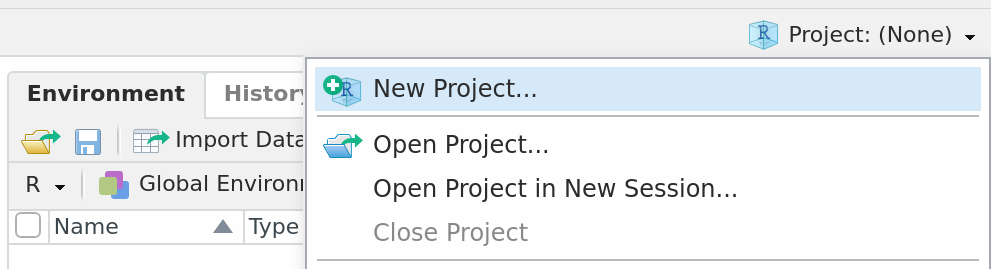
\includegraphics[width=0.85\linewidth]{https://healthinnovation.github.io/curso-introduccion-r-tidyverse/sesion_01/img/creacion_proyectos_1} \end{center}

\begin{enumerate}
\def\labelenumi{\arabic{enumi}.}
\setcounter{enumi}{1}
\tightlist
\item
  ``New Directory'' se utiliza para indicar dónde voy a almacenar mis archivos y para que R cree una nueva carpeta para mi proyecto, mientras que ``Existing Directory'' se utiliza si ya tengo una carpeta en la cual voy a almacenar mis archivos. Seleccionamos ``New Directory''.
\end{enumerate}

\begin{center}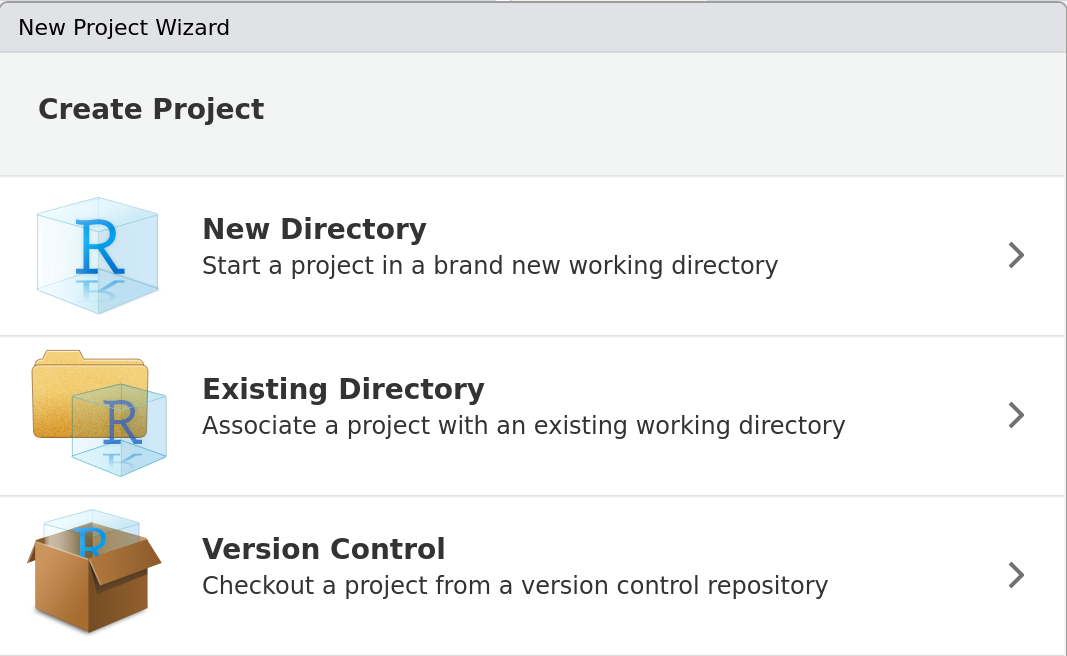
\includegraphics[width=0.85\linewidth]{https://healthinnovation.github.io/curso-introduccion-r-tidyverse/sesion_01/img/creacion_proyectos_3} \end{center}

\begin{enumerate}
\def\labelenumi{\arabic{enumi}.}
\setcounter{enumi}{2}
\tightlist
\item
  Aparecerán más opciones y seleccionamos nuevamente ``New Project''
\end{enumerate}

\begin{center}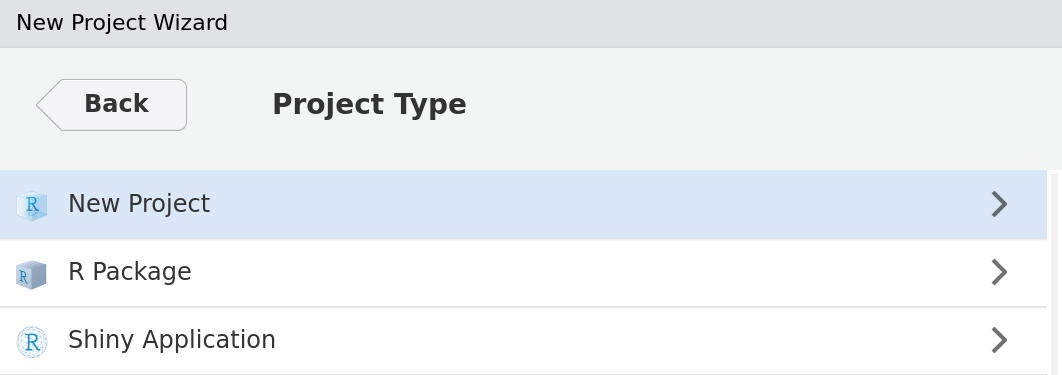
\includegraphics[width=0.85\linewidth]{https://healthinnovation.github.io/curso-introduccion-r-tidyverse/sesion_01/img/creacion_proyectos_4} \end{center}

\begin{enumerate}
\def\labelenumi{\arabic{enumi}.}
\setcounter{enumi}{2}
\tightlist
\item
  En caso de haber seleccionado ``Existing Directory'' aparecerá esto y buscamos el nombre de la carpeta que utilizaremos.
\end{enumerate}

\begin{center}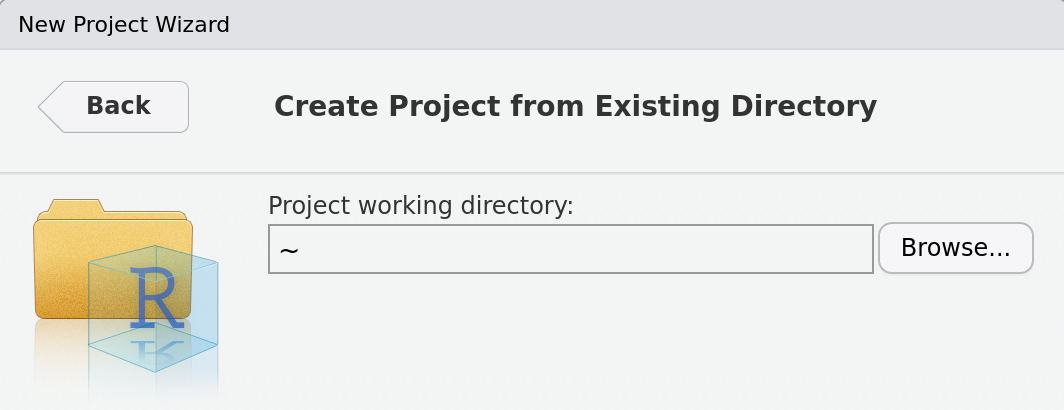
\includegraphics[width=0.85\linewidth]{https://healthinnovation.github.io/curso-introduccion-r-tidyverse/sesion_01/img/creacion_proyectos_5} \end{center}

\begin{enumerate}
\def\labelenumi{\arabic{enumi}.}
\setcounter{enumi}{3}
\tightlist
\item
  En ``Directory name'' ponemos el nombre de la carpeta que contendrá el archivo del proyecto, mientras que en ``Create project as subdirectory of'' seleccionamos dónde está la carpeta en la que trabajaremos.
\end{enumerate}

\begin{center}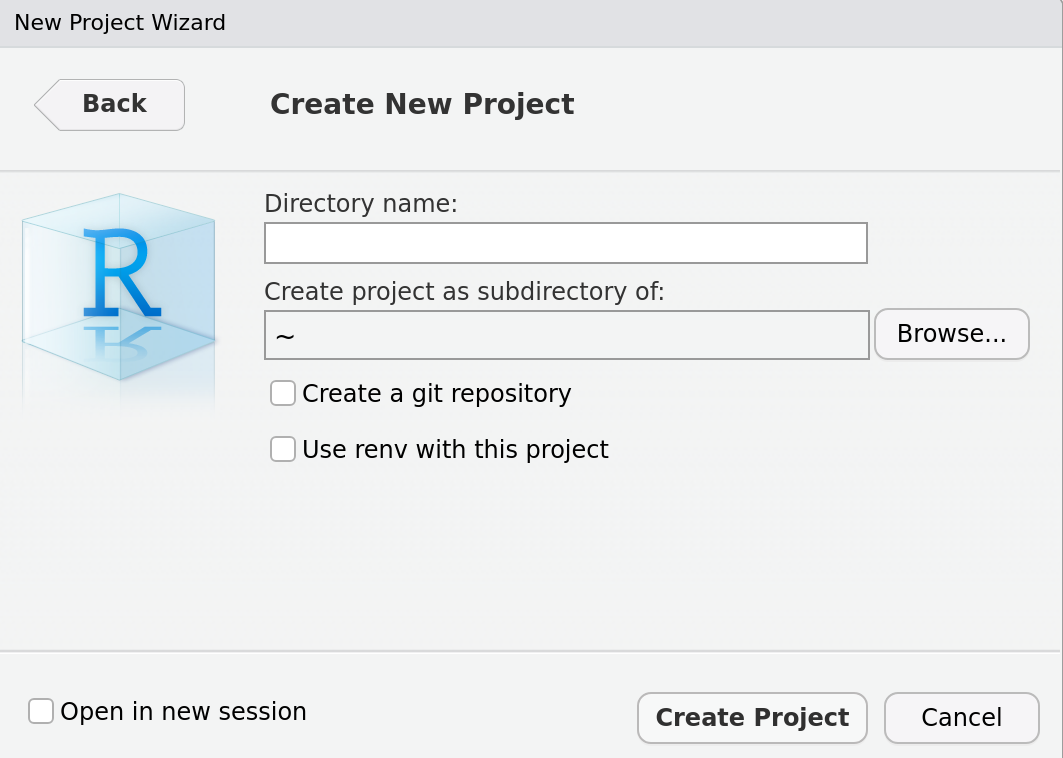
\includegraphics[width=0.85\linewidth]{https://healthinnovation.github.io/curso-introduccion-r-tidyverse/sesion_01/img/creacion_proyectos_6} \end{center}

\begin{enumerate}
\def\labelenumi{\arabic{enumi}.}
\setcounter{enumi}{4}
\tightlist
\item
  Resumen
\end{enumerate}

\begin{center}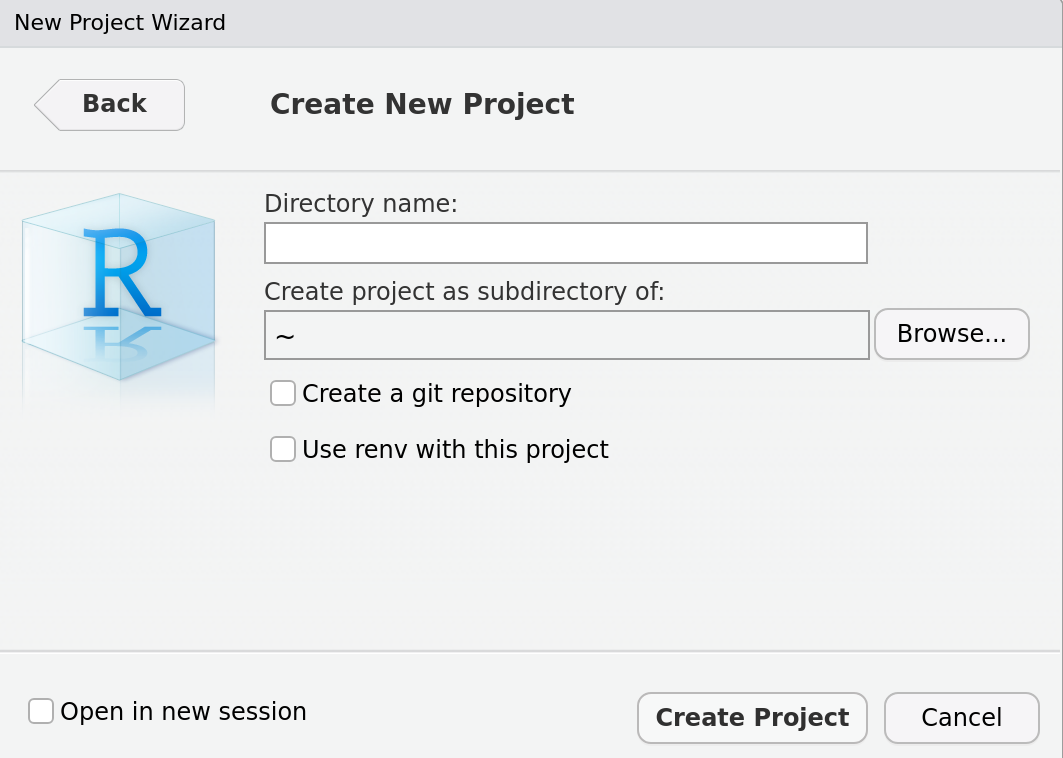
\includegraphics[width=0.85\linewidth]{https://healthinnovation.github.io/curso-introduccion-r-tidyverse/sesion_01/img/creacion_proyectos_6} \end{center}

\hypertarget{vectores-atuxf3micos}{%
\subsection{Vectores atómicos}\label{vectores-atuxf3micos}}

\begin{itemize}
\item
  Los vectores contienen información homogénea o siempre de un solo tipo de datos.
\item
  Un vector puede contener 1 solo elemento o n-elementos.
\item
  Existen hasta 6 tipos de datos que puede contener un vector:

  \begin{itemize}
  \tightlist
  \item
    Logical: \texttt{TRUE}, \texttt{FALSE}
  \item
    Integer: \texttt{1,\ 5,\ 7}
  \item
    Double: \texttt{3.15,\ 10,\ 12.86}
  \item
    Character: \texttt{"Marcos",\ "Laptop"}.
  \item
    Complex: \texttt{3\ +\ 2i}
  \end{itemize}
\end{itemize}

\textbf{Ejemplos:}

\begin{Shaded}
\begin{Highlighting}[]
\NormalTok{v\_numeric }\OtherTok{\textless{}{-}} \DecValTok{5}
\NormalTok{v\_numeric}
\CommentTok{\#\textgreater{} [1] 5}
\end{Highlighting}
\end{Shaded}

\begin{Shaded}
\begin{Highlighting}[]
\NormalTok{v\_numeric }\OtherTok{\textless{}{-}} \FunctionTok{c}\NormalTok{(}\DecValTok{5}\NormalTok{, }\DecValTok{10}\NormalTok{, }\DecValTok{15}\NormalTok{)}
\NormalTok{v\_numeric}
\CommentTok{\#\textgreater{} [1]  5 10 15}
\end{Highlighting}
\end{Shaded}

\begin{Shaded}
\begin{Highlighting}[]
\FunctionTok{typeof}\NormalTok{(v\_numeric)}
\CommentTok{\#\textgreater{} [1] "double"}
\end{Highlighting}
\end{Shaded}

\begin{Shaded}
\begin{Highlighting}[]
\NormalTok{v\_character }\OtherTok{\textless{}{-}} \FunctionTok{c}\NormalTok{(}\StringTok{"Laptop"}\NormalTok{, }\StringTok{"Rstudio"}\NormalTok{, }\StringTok{"4.2"}\NormalTok{)}
\NormalTok{v\_character}
\CommentTok{\#\textgreater{} [1] "Laptop"  "Rstudio" "4.2"}
\end{Highlighting}
\end{Shaded}

Los vectores solo pueden tener un solo tipo de información a la vez, así que si dentro de un vector se ingresa un elemento tipo numeric, este inmediatamente será transformado a character.

\begin{Shaded}
\begin{Highlighting}[]
\NormalTok{v\_character }\OtherTok{\textless{}{-}} \FunctionTok{c}\NormalTok{(}\StringTok{"Laptop"}\NormalTok{, }\StringTok{"Rstudio"}\NormalTok{, }\FloatTok{4.2}\NormalTok{)}
\NormalTok{v\_character}
\CommentTok{\#\textgreater{} [1] "Laptop"  "Rstudio" "4.2"}
\end{Highlighting}
\end{Shaded}

\begin{Shaded}
\begin{Highlighting}[]
\FunctionTok{typeof}\NormalTok{(v\_character)}
\CommentTok{\#\textgreater{} [1] "character"}
\end{Highlighting}
\end{Shaded}

Ahora crearemos 2 vectores llamados nombres y edades.

\begin{Shaded}
\begin{Highlighting}[]
\NormalTok{nombres }\OtherTok{\textless{}{-}} \FunctionTok{c}\NormalTok{(}\StringTok{"Luis"}\NormalTok{, }\StringTok{"Mateo"}\NormalTok{, }\StringTok{"Carlos"}\NormalTok{, }\StringTok{"Eduardo"}\NormalTok{)}
\NormalTok{edades }\OtherTok{\textless{}{-}} \FunctionTok{c}\NormalTok{(}\DecValTok{28}\NormalTok{, }\DecValTok{30}\NormalTok{, }\DecValTok{40}\NormalTok{, }\DecValTok{35}\NormalTok{)}
\end{Highlighting}
\end{Shaded}

A partir de esto, podemos construir algo con lo que probablemente estemos más familiarizados.

\begin{Shaded}
\begin{Highlighting}[]
\FunctionTok{data.frame}\NormalTok{(nombres, }
\NormalTok{           edades)}
\CommentTok{\#\textgreater{}   nombres edades}
\CommentTok{\#\textgreater{} 1    Luis     28}
\CommentTok{\#\textgreater{} 2   Mateo     30}
\CommentTok{\#\textgreater{} 3  Carlos     40}
\CommentTok{\#\textgreater{} 4 Eduardo     35}
\end{Highlighting}
\end{Shaded}

\hypertarget{sesiuxf3n-02}{%
\chapter{Sesión 02}\label{sesiuxf3n-02}}

\hypertarget{quuxe9-es-una-funciuxf3n}{%
\subsection{¿Qué es una función?}\label{quuxe9-es-una-funciuxf3n}}

Las funciones son módulos de código autónomo que realizan una tarea específica y generalmente, toman algún tipo de estructura de datos (vector, dataframes, etc.), lo procesan y devuelven un resultado.

El uso general de una función es el nombre de la función seguida de paréntesis

\begin{verbatim}
function_name(input)
\end{verbatim}

Los inputs se denominan argumentos e incluyen:

\begin{itemize}
\item
  El objeto físico (cualquier estructura de datos) en el que la función lleva a cabo una tarea.
\item
  Especificaciones que alteran la forma en que opera la función
\end{itemize}

\begin{center}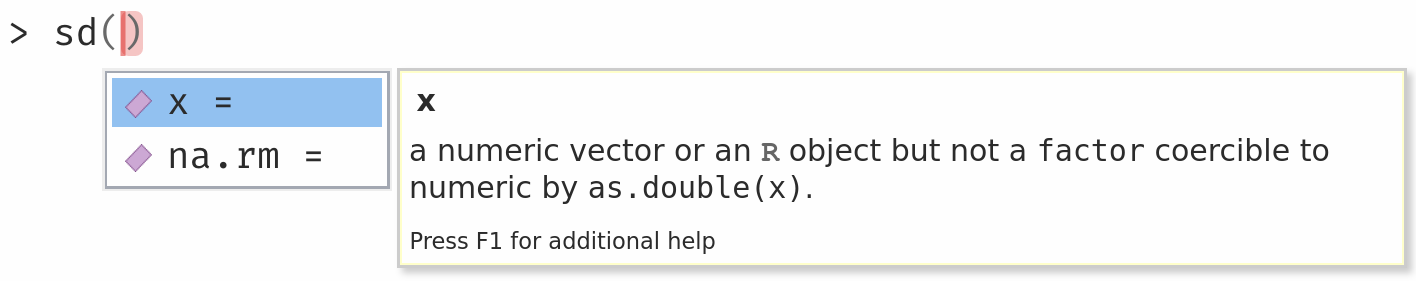
\includegraphics[width=0.85\linewidth]{https://healthinnovation.github.io/curso-introduccion-r-tidyverse/sesion_02/img/function_example} \end{center}

\hypertarget{buscando-ayuda-sobre-las-funciones}{%
\subsection{Buscando ayuda sobre las funciones}\label{buscando-ayuda-sobre-las-funciones}}

La mejor forma de averiguar esta información es utilizar ? seguido del nombre de la función. Al hacer esto, se abrirá el manual de ayuda en el panel inferior derecho de RStudio que proporcionará una descripción de la función, uso, argumentos, detalles y ejemplos:

\begin{itemize}
\tightlist
\item
  \texttt{?sd}
\item
  \texttt{help(sd)}
\item
\end{itemize}

\begin{center}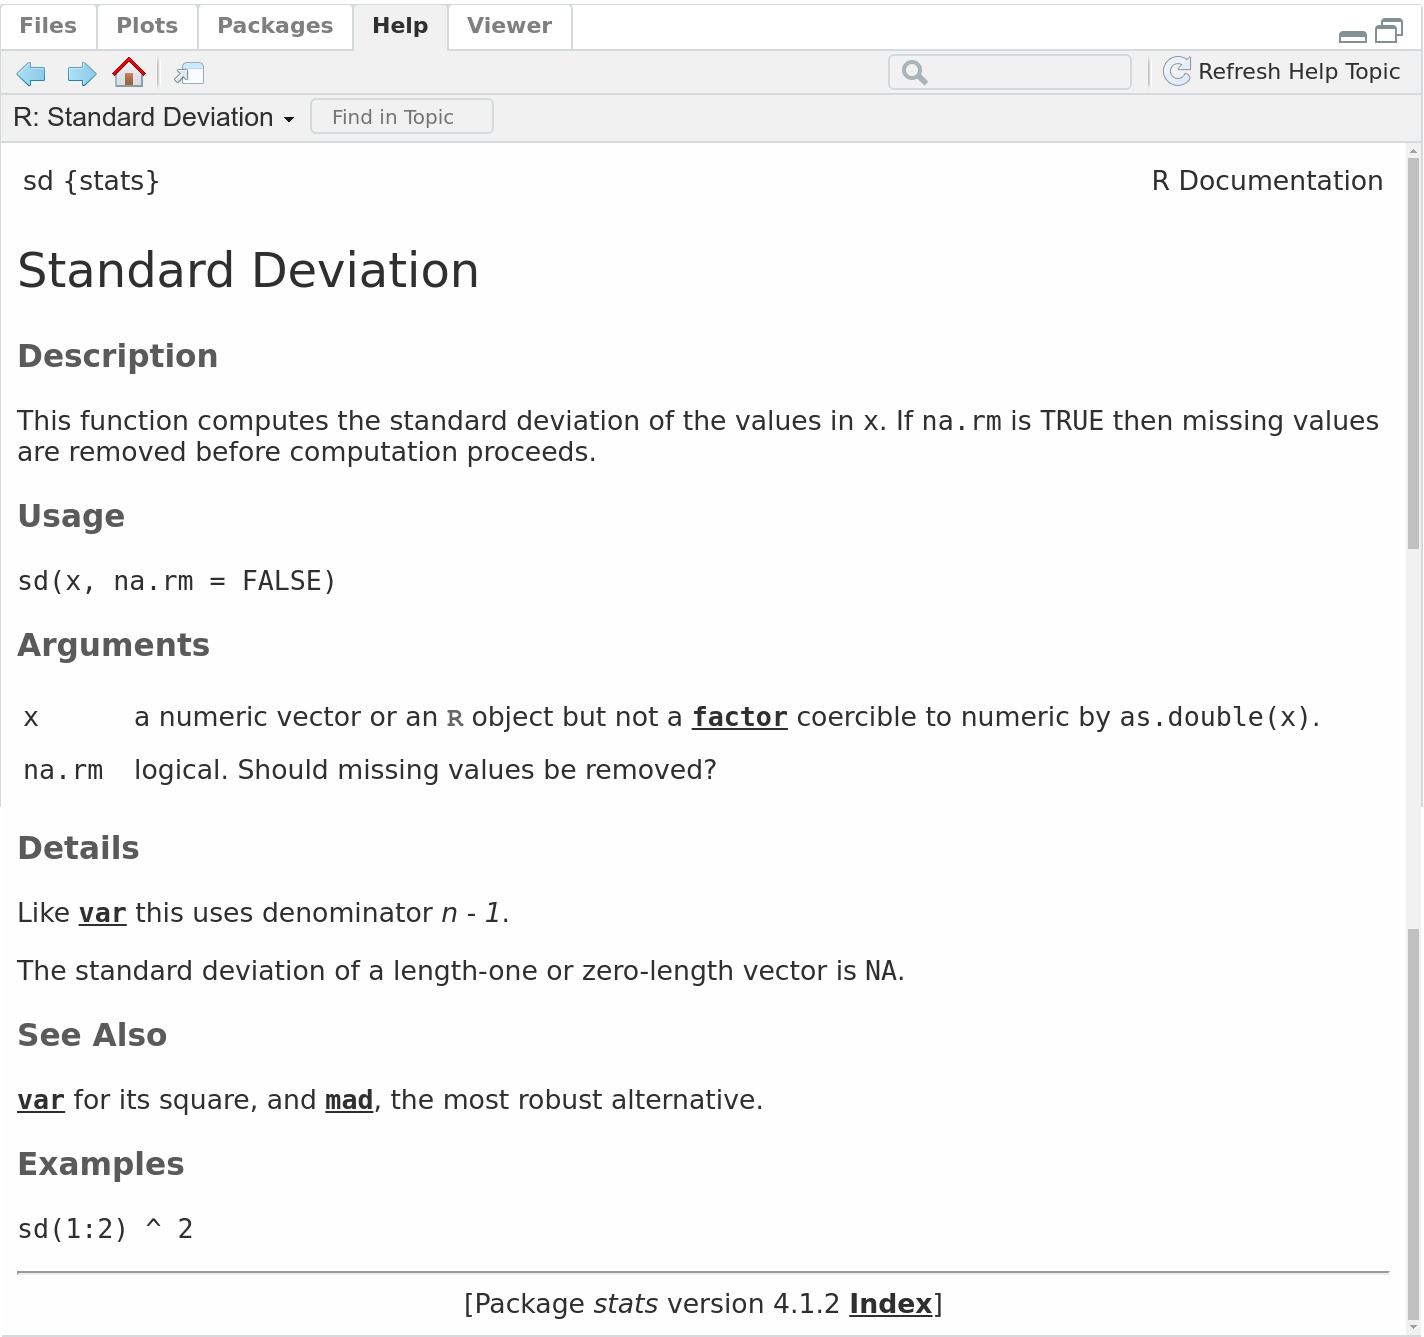
\includegraphics[width=0.85\linewidth]{https://healthinnovation.github.io/curso-introduccion-r-tidyverse/sesion_02/img/help_page} \end{center}

Alternativamente, si está familiarizado con la función pero solo necesita recordar los nombres de los argumentos, puede usar:

\begin{Shaded}
\begin{Highlighting}[]
\FunctionTok{args}\NormalTok{(sd)}
\end{Highlighting}
\end{Shaded}

\begin{verbatim}
## function (x, na.rm = FALSE) 
## NULL
\end{verbatim}

\hypertarget{ejemplo-de-una-funciuxf3n}{%
\subsection{Ejemplo de una función}\label{ejemplo-de-una-funciuxf3n}}

Se tiene el número 3.15181930, pero solo necesitamos dos decimales. Para ello, utilizaremos la función round() que redondea los números de acuerdo a la cantidad de decimales que asignemos. En este caso, solo necesitaremos 2.

\begin{Shaded}
\begin{Highlighting}[]
\FunctionTok{round}\NormalTok{(}\FloatTok{3.15181930}\NormalTok{, }\AttributeTok{digits =} \DecValTok{2}\NormalTok{)}
\CommentTok{\#\textgreater{} [1] 3.15}
\end{Highlighting}
\end{Shaded}

Como se puede observar, se ha utilizado el argumento digits para regular la cantidad de decimales.

\textbf{Nota: Si proporcionamos los argumentos en el mismo orden en el que han sido definidos, no es necesario nombrarlos}

\begin{Shaded}
\begin{Highlighting}[]
\FunctionTok{round}\NormalTok{(}\FloatTok{3.15181930}\NormalTok{, }\DecValTok{2}\NormalTok{)}
\CommentTok{\#\textgreater{} [1] 3.15}
\end{Highlighting}
\end{Shaded}

\hypertarget{data.frame}{%
\subsection{¿Data.frame?}\label{data.frame}}

\begin{itemize}
\item
  Estructura de datos 2D
\item
  Admite datos con diferente tipo de variable (lo opuesto a matrices)
\item
  Similar a Microsoft Excel
\end{itemize}

\textbf{Se crean con la función:}

\begin{verbatim}
data.frame(
  Var1 = elementos1,
  Var2 = elementos2
)
\end{verbatim}

\begin{Shaded}
\begin{Highlighting}[]
\NormalTok{var1 }\OtherTok{\textless{}{-}} \FunctionTok{c}\NormalTok{(}\StringTok{"Peru"}\NormalTok{, }\StringTok{"Argentina"}\NormalTok{, }\StringTok{"Bolivia"}\NormalTok{)}
\NormalTok{var2 }\OtherTok{\textless{}{-}} \FunctionTok{rep}\NormalTok{(}\StringTok{"aceptado"}\NormalTok{,}\DecValTok{3}\NormalTok{)}
\NormalTok{var3 }\OtherTok{\textless{}{-}} \FunctionTok{seq}\NormalTok{(}\DecValTok{1000}\NormalTok{,}\DecValTok{1200}\NormalTok{,}\DecValTok{100}\NormalTok{)}
\NormalTok{df }\OtherTok{\textless{}{-}} \FunctionTok{data.frame}\NormalTok{(var1, var2, var3)}
\NormalTok{df}
\CommentTok{\#\textgreater{}        var1     var2 var3}
\CommentTok{\#\textgreater{} 1      Peru aceptado 1000}
\CommentTok{\#\textgreater{} 2 Argentina aceptado 1100}
\CommentTok{\#\textgreater{} 3   Bolivia aceptado 1200}
\end{Highlighting}
\end{Shaded}

\begin{Shaded}
\begin{Highlighting}[]
\NormalTok{df }\OtherTok{\textless{}{-}} \FunctionTok{data.frame}\NormalTok{(}
  \AttributeTok{var1 =} \FunctionTok{c}\NormalTok{(}\StringTok{"Peru"}\NormalTok{, }\StringTok{"Argentina"}\NormalTok{, }\StringTok{"Bolivia"}\NormalTok{),}
  \AttributeTok{var2 =} \FunctionTok{rep}\NormalTok{(}\StringTok{"aceptado"}\NormalTok{,}\DecValTok{3}\NormalTok{),}
  \AttributeTok{var3 =} \FunctionTok{seq}\NormalTok{(}\DecValTok{1000}\NormalTok{,}\DecValTok{1200}\NormalTok{,}\DecValTok{100}\NormalTok{)}
\NormalTok{)}
\NormalTok{df}
\CommentTok{\#\textgreater{}        var1     var2 var3}
\CommentTok{\#\textgreater{} 1      Peru aceptado 1000}
\CommentTok{\#\textgreater{} 2 Argentina aceptado 1100}
\CommentTok{\#\textgreater{} 3   Bolivia aceptado 1200}
\end{Highlighting}
\end{Shaded}

\hypertarget{tibble}{%
\subsection{¿Tibble?}\label{tibble}}

\begin{itemize}
\tightlist
\item
  Son la versión mejorada del data.frame
\item
  Disponible en el paquete tibble y por lo tanto en el tidyverse.
\end{itemize}

\textbf{Se crean con la función:}

\begin{verbatim}
# Instalación
install.packages("tibble")
# Llavado o activación de paquete
library(tibble)
tibble(
  Var1 = elementos1,
  Var2 = elementos2
)
\end{verbatim}

\begin{Shaded}
\begin{Highlighting}[]
\FunctionTok{library}\NormalTok{(tibble)}
\FunctionTok{tibble}\NormalTok{(}
  \AttributeTok{var1 =} \FunctionTok{c}\NormalTok{(}\StringTok{"Peru"}\NormalTok{, }\StringTok{"Argentina"}\NormalTok{, }\StringTok{"Bolivia"}\NormalTok{),}
  \AttributeTok{var2 =} \FunctionTok{rep}\NormalTok{(}\StringTok{"aceptado"}\NormalTok{,}\DecValTok{3}\NormalTok{),}
  \AttributeTok{var3 =} \FunctionTok{seq}\NormalTok{(}\DecValTok{1000}\NormalTok{,}\DecValTok{1200}\NormalTok{,}\DecValTok{100}\NormalTok{)}
\NormalTok{)}
\CommentTok{\#\textgreater{} \# A tibble: 3 x 3}
\CommentTok{\#\textgreater{}   var1      var2      var3}
\CommentTok{\#\textgreater{}   \textless{}chr\textgreater{}     \textless{}chr\textgreater{}    \textless{}dbl\textgreater{}}
\CommentTok{\#\textgreater{} 1 Peru      aceptado  1000}
\CommentTok{\#\textgreater{} 2 Argentina aceptado  1100}
\CommentTok{\#\textgreater{} 3 Bolivia   aceptado  1200}
\end{Highlighting}
\end{Shaded}

\hypertarget{data.frame-v.s.-tibble}{%
\subsection{data.frame() v.s. tibble()}\label{data.frame-v.s.-tibble}}

Ambas funciones tienen sus versiones \texttt{as.*} o \texttt{as\_*} que permite transformar algo en lo que se desea. En este caso se estaría usando as.data.frame para convertir algo a data.frame y as\_tibble para ese mismo objetivo.

\begin{Shaded}
\begin{Highlighting}[]
\FunctionTok{class}\NormalTok{(iris)}
\CommentTok{\#\textgreater{} [1] "data.frame"}
\end{Highlighting}
\end{Shaded}

\begin{Shaded}
\begin{Highlighting}[]
\CommentTok{\# data.frame}
\FunctionTok{head}\NormalTok{(iris) }\CommentTok{\# Muestra las 6 primeras filas del data.frame}
\CommentTok{\#\textgreater{}   Sepal.Length Sepal.Width Petal.Length Petal.Width Species}
\CommentTok{\#\textgreater{} 1          5.1         3.5          1.4         0.2  setosa}
\CommentTok{\#\textgreater{} 2          4.9         3.0          1.4         0.2  setosa}
\CommentTok{\#\textgreater{} 3          4.7         3.2          1.3         0.2  setosa}
\CommentTok{\#\textgreater{} 4          4.6         3.1          1.5         0.2  setosa}
\CommentTok{\#\textgreater{} 5          5.0         3.6          1.4         0.2  setosa}
\CommentTok{\#\textgreater{} 6          5.4         3.9          1.7         0.4  setosa}
\end{Highlighting}
\end{Shaded}

\begin{Shaded}
\begin{Highlighting}[]
\CommentTok{\# tibble}
\FunctionTok{as\_tibble}\NormalTok{(iris)}
\CommentTok{\#\textgreater{} \# A tibble: 150 x 5}
\CommentTok{\#\textgreater{}    Sepal.Length Sepal.Width Petal.Length Petal.Width Species}
\CommentTok{\#\textgreater{}           \textless{}dbl\textgreater{}       \textless{}dbl\textgreater{}        \textless{}dbl\textgreater{}       \textless{}dbl\textgreater{} \textless{}fct\textgreater{}  }
\CommentTok{\#\textgreater{}  1          5.1         3.5          1.4         0.2 setosa }
\CommentTok{\#\textgreater{}  2          4.9         3            1.4         0.2 setosa }
\CommentTok{\#\textgreater{}  3          4.7         3.2          1.3         0.2 setosa }
\CommentTok{\#\textgreater{}  4          4.6         3.1          1.5         0.2 setosa }
\CommentTok{\#\textgreater{}  5          5           3.6          1.4         0.2 setosa }
\CommentTok{\#\textgreater{}  6          5.4         3.9          1.7         0.4 setosa }
\CommentTok{\#\textgreater{}  7          4.6         3.4          1.4         0.3 setosa }
\CommentTok{\#\textgreater{}  8          5           3.4          1.5         0.2 setosa }
\CommentTok{\#\textgreater{}  9          4.4         2.9          1.4         0.2 setosa }
\CommentTok{\#\textgreater{} 10          4.9         3.1          1.5         0.1 setosa }
\CommentTok{\#\textgreater{} \# ... with 140 more rows}
\end{Highlighting}
\end{Shaded}

\hypertarget{quuxe9-es-un-paquete}{%
\subsection{¿Qué es un paquete?}\label{quuxe9-es-un-paquete}}

Los paquetes son colecciones de funciones, datos y código compilado de R en un formato bien definido, creados para agregar una funcionalidad específica.

Hay un conjunto de paquetes estándar (o base) que se consideran parte del código fuente de R y están disponibles automáticamente como parte de su instalación de R.

\begin{center}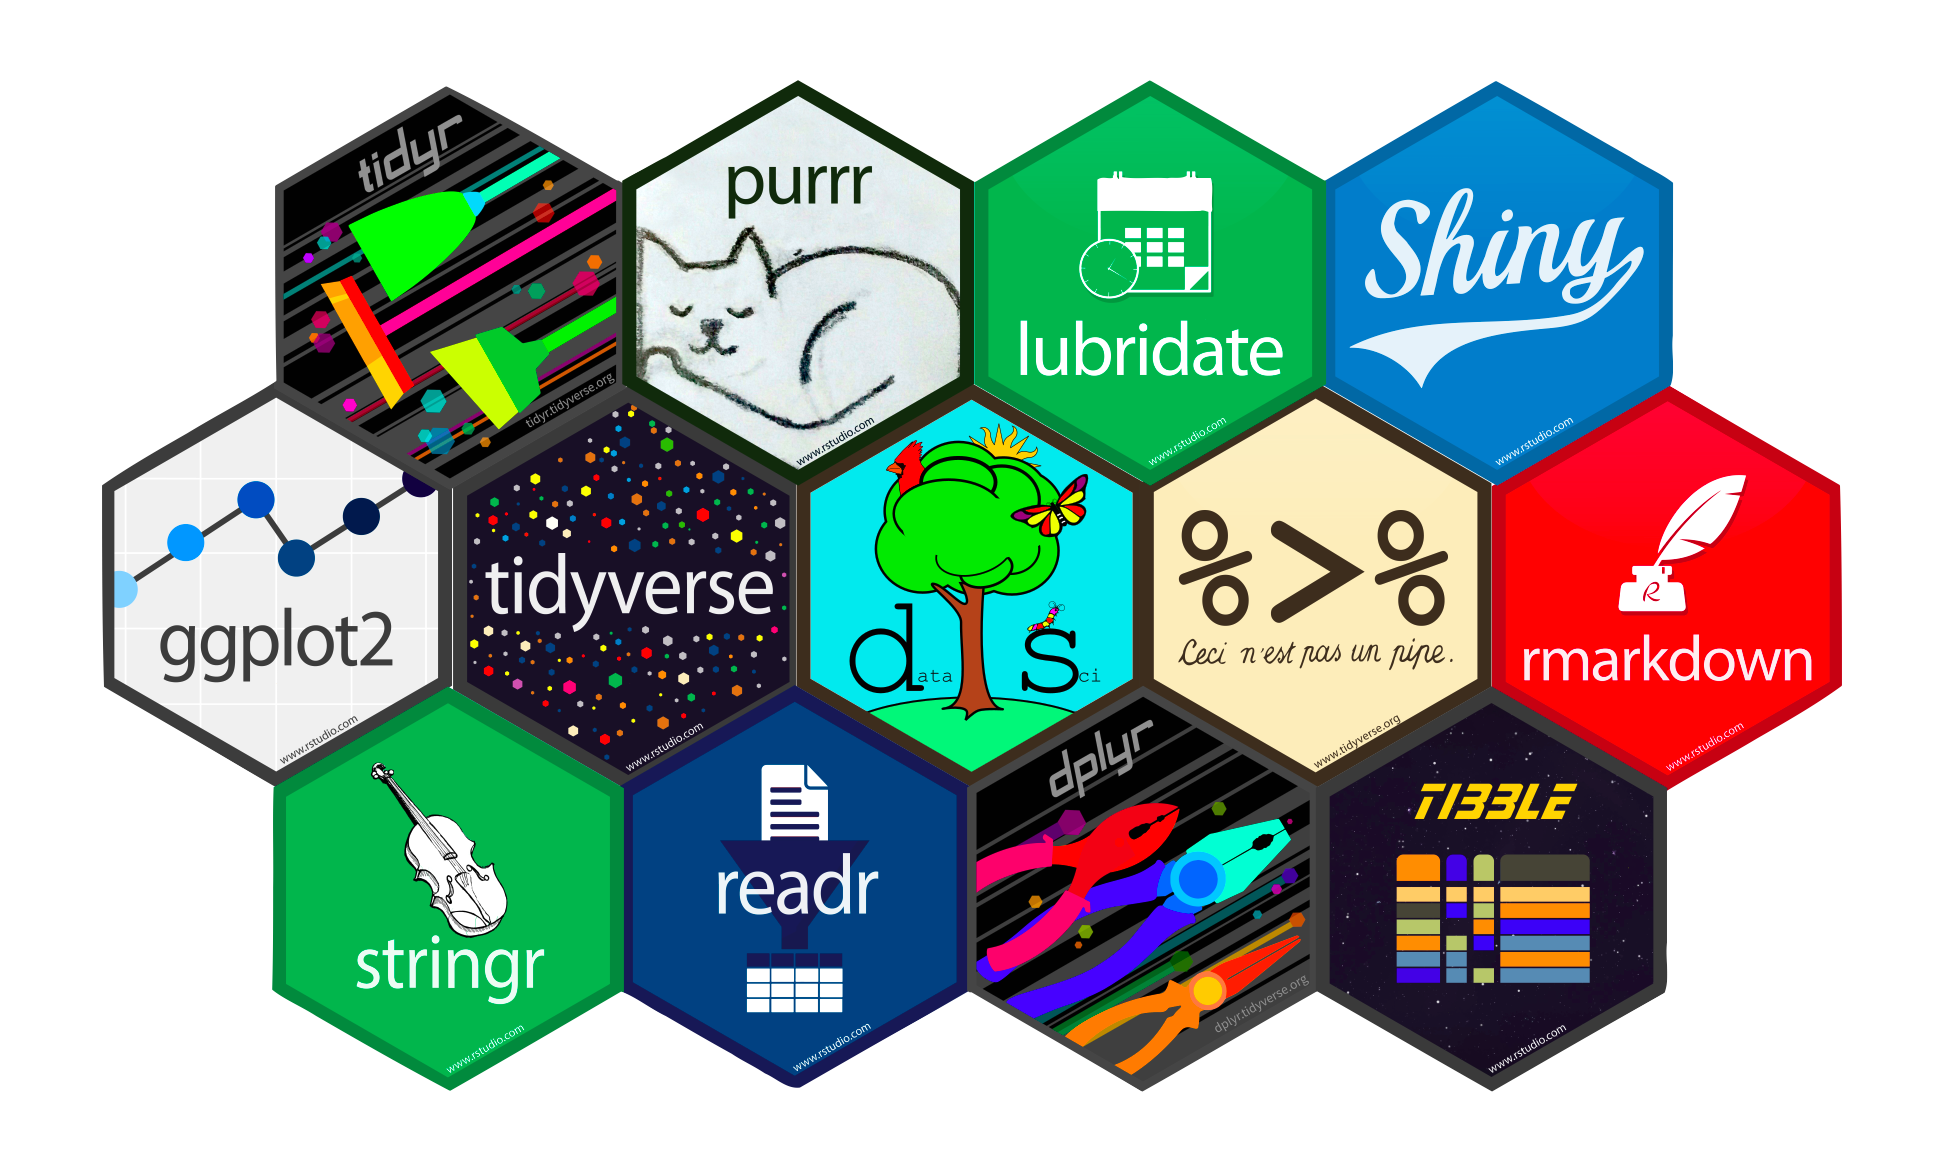
\includegraphics[width=0.85\linewidth]{https://healthinnovation.github.io/curso-introduccion-r-tidyverse/sesion_02/img/paquetes_hexa} \end{center}

\hypertarget{instalaciuxf3n-de-paquetes-desde-cran}{%
\subsection{Instalación de paquetes desde CRAN}\label{instalaciuxf3n-de-paquetes-desde-cran}}

La forma de instalar un paquete dependerá de dónde se encuentre. Entonces, para los paquetes disponibles públicamente, esto significa a qué repositorio pertenece. La forma más común es usar el repositorio CRAN, luego solo necesita el nombre del paquete y usa el siguiente comando:

\begin{Shaded}
\begin{Highlighting}[]
\FunctionTok{install.packages}\NormalTok{(}\StringTok{"paquete"}\NormalTok{)}
\end{Highlighting}
\end{Shaded}

Después de ejecutar esto, recibirá algunos mensajes en la pantalla. Dependerán del sistema operativo que esté utilizando, las dependencias y si el paquete se instaló correctamente.

\hypertarget{instalaciuxf3n-de-paquetes-vuxeda-remotes}{%
\subsection{Instalación de paquetes vía remotes}\label{instalaciuxf3n-de-paquetes-vuxeda-remotes}}

Cada repositorio tiene su propia forma de instalar un paquete a partir de ellos, por lo que en el caso de que utilice regularmente paquetes de diferentes fuentes, este comportamiento puede ser un poco frustrante. Una forma más eficiente es probablemente usar el paquete \texttt{remotes} para simplificar este proceso.

\begin{Shaded}
\begin{Highlighting}[]
\FunctionTok{install.packages}\NormalTok{(}\StringTok{"remotes"}\NormalTok{)}
\end{Highlighting}
\end{Shaded}

Después de haber instalado \texttt{remotes} podemos utilizar algunas de sus funciones para la instalación de paquetes:

\begin{itemize}
\item
  \texttt{remotes::install\_bioc()} desde Bioconductor
\item
  \texttt{remotes::install\_github()} desde GitHub
\item
  \texttt{remotes::install\_version()} para instalar una versión específica de CRAN.
\end{itemize}

\hypertarget{bases-de-datos-a-utilizar}{%
\subsection{Bases de datos a utilizar}\label{bases-de-datos-a-utilizar}}

Usaremos una base de datos proporcionado por \href{https://www.nature.com/articles/s41598-018-27482-2}{Gan et al.~(2018)} en su estudio:

Dicho estudio es un ensayo clínico aleatorizado (ECA) de 400 participantes en el que se compara 2 tipos de tratamientos para erradicar la infección por Helicobácter Pylori.

\begin{itemize}
\item
  \textbf{Grupo A de tratamiento}: Esomeprazol, amoxicilina, bismuto coloidal con pectina y levofloxacina 500mg una vez al día.
\item
  \textbf{Grupo B de tratamiento}: Levofloxacina 200mg dos veces al día, durante un periodo de 14 días.
\end{itemize}

Randomized group

n

group A

200

group B

200

\hypertarget{importaciuxf3n-de-datos-i}{%
\subsection{Importación de datos I}\label{importaciuxf3n-de-datos-i}}

\begin{longtable}[]{@{}
  >{\raggedright\arraybackslash}p{(\columnwidth - 2\tabcolsep) * \real{0.5385}}
  >{\raggedright\arraybackslash}p{(\columnwidth - 2\tabcolsep) * \real{0.4615}}@{}}
\toprule
\begin{minipage}[b]{\linewidth}\raggedright
Función
\end{minipage} & \begin{minipage}[b]{\linewidth}\raggedright
Archivos
\end{minipage} \\
\midrule
\endhead
\texttt{readxl::read\_excel()} & \\
\texttt{readr::read\_csv()} & \\
\texttt{haven::read\_dta()} & \\
\texttt{haven::read\_sav()} & \\
\bottomrule
\end{longtable}

Vamos a importar el archivo excel que tiene una extensión \texttt{.xlsx} y se encuentra dentro de la carpeta data.

\textbf{Recuerda:} \emph{Al importar el archivo debemos asignarlo a un objeto, para poder guardar la información. En este caso llamaremos a este objeto como \texttt{trial\_data}.}

\begin{verbatim}
#> -- Attaching packages -------------------------------------------------------------------------- tidyverse 1.3.1 --
#> v ggplot2 3.3.6     v dplyr   1.0.9
#> v tidyr   1.2.0     v stringr 1.4.0
#> v readr   2.1.2     v forcats 0.5.1
#> v purrr   0.3.4
#> -- Conflicts ----------------------------------------------------------------------------- tidyverse_conflicts() --
#> x dplyr::filter() masks stats::filter()
#> x dplyr::lag()    masks stats::lag()
\end{verbatim}

\begin{Shaded}
\begin{Highlighting}[]
\NormalTok{trial\_data }\OtherTok{\textless{}{-}}\NormalTok{ readxl}\SpecialCharTok{::}\FunctionTok{read\_excel}\NormalTok{(}\StringTok{"\_data/researchdata.xlsx"}\NormalTok{)}
\NormalTok{trial\_data}
\CommentTok{\#\textgreater{} \# A tibble: 400 x 10}
\CommentTok{\#\textgreater{}    \textasciigrave{}Patient number\textasciigrave{} \textasciigrave{}Baseline 13C{-}UBT\textasciigrave{} \textasciigrave{}Randomized group\textasciigrave{}}
\CommentTok{\#\textgreater{}               \textless{}dbl\textgreater{} \textless{}chr\textgreater{}              \textless{}chr\textgreater{}             }
\CommentTok{\#\textgreater{}  1                1 Positive           group B           }
\CommentTok{\#\textgreater{}  2                2 Positive           group A           }
\CommentTok{\#\textgreater{}  3                3 Positive           group B           }
\CommentTok{\#\textgreater{}  4                4 Positive           group A           }
\CommentTok{\#\textgreater{}  5                5 Positive           group A           }
\CommentTok{\#\textgreater{}  6                6 Positive           group A           }
\CommentTok{\#\textgreater{}  7                7 Positive           group B           }
\CommentTok{\#\textgreater{}  8                8 Positive           group A           }
\CommentTok{\#\textgreater{}  9                9 Positive           group A           }
\CommentTok{\#\textgreater{} 10               10 Positive           group A           }
\CommentTok{\#\textgreater{} \# ... with 390 more rows, and 7 more variables:}
\CommentTok{\#\textgreater{} \#   \textasciigrave{}Follow{-}up13C{-}UBT (4 weeks after therapy)\textasciigrave{} \textless{}chr\textgreater{},}
\CommentTok{\#\textgreater{} \#   \textasciigrave{}adverse drug reactions\textasciigrave{} \textless{}chr\textgreater{},}
\CommentTok{\#\textgreater{} \#   \textasciigrave{}adverse drug reactions  content\textasciigrave{} \textless{}chr\textgreater{},}
\CommentTok{\#\textgreater{} \#   \textasciigrave{}Adverse drug reaction classified\textasciigrave{} \textless{}chr\textgreater{},}
\CommentTok{\#\textgreater{} \#   \textasciigrave{}Complete the study\textasciigrave{} \textless{}chr\textgreater{}, \textasciigrave{}Uncompleted Reason\textasciigrave{} \textless{}chr\textgreater{},}
\CommentTok{\#\textgreater{} \#   \textasciigrave{}per protocol analysis\textasciigrave{} \textless{}chr\textgreater{}}
\end{Highlighting}
\end{Shaded}

\hypertarget{importaciuxf3n-de-datos-ii}{%
\subsection{Importación de datos II}\label{importaciuxf3n-de-datos-ii}}

En algunos casos estaremos frente a base de datos que contengan cierta información en sus primeras filas que no sean relevantes como datos a considerar para el análisis. La mayor cantidad de veces tienen un propósito meramente informativo. Ejemplo:

\hypertarget{situaciuxf3n}{%
\subsubsection{Situación}\label{situaciuxf3n}}

En estas situaciones tenemos 2 alternativas:

\textbf{a)} Editar el archivo en cuestión y eliminar las filas que no sean relevantes.

\textbf{b)} Durante la importación indicar que se omitan las primeras filas o filtrarlas una vez se haya importado.

Siempre será una mejor opción manejar los cambios desde el código, ya que se esa manera mantenemos los archivos originales y además podemos tener un registro de los cambios realizados.

Para hacer esto usaremos el argumento skip dentro de la función \texttt{readxl::read\_excel()}, que indicará la cantidad de filas que deseamos omitir en la importación.

\hypertarget{problema}{%
\subsubsection{Problema}\label{problema}}

Si intentamos importar la data sin especificar ningún argumento, veremos como se registran informaciones que no requerimos, y solo se encuentran en los datos a manera de información.

\begin{Shaded}
\begin{Highlighting}[]
\NormalTok{trial\_data2 }\OtherTok{\textless{}{-}}\NormalTok{ readxl}\SpecialCharTok{::}\FunctionTok{read\_excel}\NormalTok{(}\StringTok{"\_data/researchdata2.xlsx"}\NormalTok{)}
\CommentTok{\#\textgreater{} New names:}
\CommentTok{\#\textgreater{} * \textasciigrave{}\textasciigrave{} {-}\textgreater{} \textasciigrave{}...1\textasciigrave{}}
\CommentTok{\#\textgreater{} * \textasciigrave{}\textasciigrave{} {-}\textgreater{} \textasciigrave{}...3\textasciigrave{}}
\CommentTok{\#\textgreater{} * \textasciigrave{}\textasciigrave{} {-}\textgreater{} \textasciigrave{}...4\textasciigrave{}}
\CommentTok{\#\textgreater{} * \textasciigrave{}\textasciigrave{} {-}\textgreater{} \textasciigrave{}...5\textasciigrave{}}
\CommentTok{\#\textgreater{} * \textasciigrave{}\textasciigrave{} {-}\textgreater{} \textasciigrave{}...6\textasciigrave{}}
\CommentTok{\#\textgreater{} * \textasciigrave{}\textasciigrave{} {-}\textgreater{} \textasciigrave{}...7\textasciigrave{}}
\CommentTok{\#\textgreater{} * \textasciigrave{}\textasciigrave{} {-}\textgreater{} \textasciigrave{}...8\textasciigrave{}}
\CommentTok{\#\textgreater{} * \textasciigrave{}\textasciigrave{} {-}\textgreater{} \textasciigrave{}...9\textasciigrave{}}
\CommentTok{\#\textgreater{} * \textasciigrave{}\textasciigrave{} {-}\textgreater{} \textasciigrave{}...10\textasciigrave{}}
\NormalTok{trial\_data2}
\CommentTok{\#\textgreater{} \# A tibble: 403 x 10}
\CommentTok{\#\textgreater{}    ...1       \textasciigrave{}Data de ejemp\textasciitilde{}\textasciigrave{} ...3  ...4  ...5  ...6  ...7 }
\CommentTok{\#\textgreater{}    \textless{}chr\textgreater{}      \textless{}chr\textgreater{}            \textless{}chr\textgreater{} \textless{}chr\textgreater{} \textless{}chr\textgreater{} \textless{}chr\textgreater{} \textless{}chr\textgreater{}}
\CommentTok{\#\textgreater{}  1 \textless{}NA\textgreater{}       \textless{}NA\textgreater{}             \textless{}NA\textgreater{}  \textless{}NA\textgreater{}  \textless{}NA\textgreater{}  \textless{}NA\textgreater{}  \textless{}NA\textgreater{} }
\CommentTok{\#\textgreater{}  2 \textless{}NA\textgreater{}       \textless{}NA\textgreater{}             \textless{}NA\textgreater{}  \textless{}NA\textgreater{}  \textless{}NA\textgreater{}  \textless{}NA\textgreater{}  \textless{}NA\textgreater{} }
\CommentTok{\#\textgreater{}  3 Patient n\textasciitilde{} Baseline 13C{-}UBT Rand\textasciitilde{} Foll\textasciitilde{} adve\textasciitilde{} adve\textasciitilde{} Adve\textasciitilde{}}
\CommentTok{\#\textgreater{}  4 1          Positive         grou\textasciitilde{} Nega\textasciitilde{} No    NA    NA   }
\CommentTok{\#\textgreater{}  5 2          Positive         grou\textasciitilde{} Nega\textasciitilde{} Yes   Fati\textasciitilde{} Mild }
\CommentTok{\#\textgreater{}  6 3          Positive         grou\textasciitilde{} Nega\textasciitilde{} No    NA    NA   }
\CommentTok{\#\textgreater{}  7 4          Positive         grou\textasciitilde{} Posi\textasciitilde{} Yes   Abdo\textasciitilde{} Mild }
\CommentTok{\#\textgreater{}  8 5          Positive         grou\textasciitilde{} Nega\textasciitilde{} Yes   Drow\textasciitilde{} Mild }
\CommentTok{\#\textgreater{}  9 6          Positive         grou\textasciitilde{} Nega\textasciitilde{} No    NA    NA   }
\CommentTok{\#\textgreater{} 10 7          Positive         grou\textasciitilde{} Nega\textasciitilde{} No    NA    NA   }
\CommentTok{\#\textgreater{} \# ... with 393 more rows, and 3 more variables: ...8 \textless{}chr\textgreater{},}
\CommentTok{\#\textgreater{} \#   ...9 \textless{}chr\textgreater{}, ...10 \textless{}chr\textgreater{}}
\end{Highlighting}
\end{Shaded}

\hypertarget{soluciuxf3n}{%
\subsubsection{Solución}\label{soluciuxf3n}}

Ya que en este caso la base de datos llamada researchdata2.xlsx empieza a mostrar datos relevantes a partir de la fila 4, requeriremos omitir o saltar (skip) 3 filas, se la siguiente manera:

\begin{Shaded}
\begin{Highlighting}[]
\NormalTok{trial\_data2 }\OtherTok{\textless{}{-}}\NormalTok{ readxl}\SpecialCharTok{::}\FunctionTok{read\_excel}\NormalTok{(}
  \StringTok{"\_data/researchdata2.xlsx"}\NormalTok{,}
  \AttributeTok{skip =} \DecValTok{3}
\NormalTok{  )}

\NormalTok{trial\_data2}
\CommentTok{\#\textgreater{} \# A tibble: 400 x 10}
\CommentTok{\#\textgreater{}    \textasciigrave{}Patient number\textasciigrave{} \textasciigrave{}Baseline 13C{-}UBT\textasciigrave{} \textasciigrave{}Randomized group\textasciigrave{}}
\CommentTok{\#\textgreater{}               \textless{}dbl\textgreater{} \textless{}chr\textgreater{}              \textless{}chr\textgreater{}             }
\CommentTok{\#\textgreater{}  1                1 Positive           group B           }
\CommentTok{\#\textgreater{}  2                2 Positive           group A           }
\CommentTok{\#\textgreater{}  3                3 Positive           group B           }
\CommentTok{\#\textgreater{}  4                4 Positive           group A           }
\CommentTok{\#\textgreater{}  5                5 Positive           group A           }
\CommentTok{\#\textgreater{}  6                6 Positive           group A           }
\CommentTok{\#\textgreater{}  7                7 Positive           group B           }
\CommentTok{\#\textgreater{}  8                8 Positive           group A           }
\CommentTok{\#\textgreater{}  9                9 Positive           group A           }
\CommentTok{\#\textgreater{} 10               10 Positive           group A           }
\CommentTok{\#\textgreater{} \# ... with 390 more rows, and 7 more variables:}
\CommentTok{\#\textgreater{} \#   \textasciigrave{}Follow{-}up13C{-}UBT (4 weeks after therapy)\textasciigrave{} \textless{}chr\textgreater{},}
\CommentTok{\#\textgreater{} \#   \textasciigrave{}adverse drug reactions\textasciigrave{} \textless{}chr\textgreater{},}
\CommentTok{\#\textgreater{} \#   \textasciigrave{}adverse drug reactions  content\textasciigrave{} \textless{}chr\textgreater{},}
\CommentTok{\#\textgreater{} \#   \textasciigrave{}Adverse drug reaction classified\textasciigrave{} \textless{}chr\textgreater{},}
\CommentTok{\#\textgreater{} \#   \textasciigrave{}Complete the study\textasciigrave{} \textless{}chr\textgreater{}, \textasciigrave{}Uncompleted Reason\textasciigrave{} \textless{}chr\textgreater{},}
\CommentTok{\#\textgreater{} \#   \textasciigrave{}per protocol analysis\textasciigrave{} \textless{}chr\textgreater{}}
\end{Highlighting}
\end{Shaded}

\hypertarget{sesiuxf3n-03}{%
\chapter{Sesión 03}\label{sesiuxf3n-03}}

\hypertarget{funciuxf3n-glimpse}{%
\subsection{Función Glimpse}\label{funciuxf3n-glimpse}}

Mediante la función:

\begin{Shaded}
\begin{Highlighting}[]
\FunctionTok{glimpse}\NormalTok{()}
\end{Highlighting}
\end{Shaded}

\hypertarget{para-que-sirve}{%
\subsubsection{¿Para que sirve?}\label{para-que-sirve}}

\begin{itemize}
\item
  Versión transpuesta de print
\item
  Ayuda a visualizar la mayor cantidad de datos de muchas columnas.
\item
  Muestra el nombre de la variable junto con una designación de tipo de variable.
\end{itemize}

\emph{\textbf{Observación:}}

\begin{itemize}
\tightlist
\item
  Recordar importar el paquete tidyverse:
\end{itemize}

\begin{Shaded}
\begin{Highlighting}[]
\FunctionTok{library}\NormalTok{(tidyverse)}
\CommentTok{\#\textgreater{} {-}{-} Attaching packages {-}{-}{-}{-}{-}{-}{-}{-}{-}{-}{-}{-}{-}{-}{-}{-}{-}{-}{-}{-}{-}{-}{-}{-}{-}{-}{-}{-}{-}{-}{-}{-}{-}{-}{-}{-}{-}{-}{-}{-}{-}{-}{-}{-}{-}{-}{-}{-}{-}{-}{-}{-}{-}{-}{-}{-}{-}{-}{-}{-}{-}{-}{-}{-}{-}{-}{-}{-}{-}{-}{-}{-}{-}{-} tidyverse 1.3.1 {-}{-}}
\CommentTok{\#\textgreater{} v ggplot2 3.3.6     v purrr   0.3.4}
\CommentTok{\#\textgreater{} v tibble  3.1.7     v dplyr   1.0.9}
\CommentTok{\#\textgreater{} v tidyr   1.2.0     v stringr 1.4.0}
\CommentTok{\#\textgreater{} v readr   2.1.2     v forcats 0.5.1}
\CommentTok{\#\textgreater{} {-}{-} Conflicts {-}{-}{-}{-}{-}{-}{-}{-}{-}{-}{-}{-}{-}{-}{-}{-}{-}{-}{-}{-}{-}{-}{-}{-}{-}{-}{-}{-}{-}{-}{-}{-}{-}{-}{-}{-}{-}{-}{-}{-}{-}{-}{-}{-}{-}{-}{-}{-}{-}{-}{-}{-}{-}{-}{-}{-}{-}{-}{-}{-}{-}{-}{-}{-}{-}{-}{-}{-}{-}{-}{-}{-}{-}{-}{-}{-}{-} tidyverse\_conflicts() {-}{-}}
\CommentTok{\#\textgreater{} x dplyr::filter() masks stats::filter()}
\CommentTok{\#\textgreater{} x dplyr::lag()    masks stats::lag()}
\FunctionTok{library}\NormalTok{(dplyr)}
\end{Highlighting}
\end{Shaded}

\begin{itemize}
\tightlist
\item
  Para el ejemplo se recomienda installar el siguiente paquete:
\end{itemize}

\begin{Shaded}
\begin{Highlighting}[]
\FunctionTok{install.packages}\NormalTok{(}\StringTok{"nycflights13"}\NormalTok{)}
\end{Highlighting}
\end{Shaded}

\hypertarget{ejemplo}{%
\subsubsection{Ejemplo}\label{ejemplo}}

Así habitualmente observamos la data:

\begin{Shaded}
\begin{Highlighting}[]
\NormalTok{nycflights13}\SpecialCharTok{::}\NormalTok{flights}
\CommentTok{\#\textgreater{} \# A tibble: 336,776 x 19}
\CommentTok{\#\textgreater{}     year month   day dep\_time sched\_dep\_time dep\_delay}
\CommentTok{\#\textgreater{}    \textless{}int\textgreater{} \textless{}int\textgreater{} \textless{}int\textgreater{}    \textless{}int\textgreater{}          \textless{}int\textgreater{}     \textless{}dbl\textgreater{}}
\CommentTok{\#\textgreater{}  1  2013     1     1      517            515         2}
\CommentTok{\#\textgreater{}  2  2013     1     1      533            529         4}
\CommentTok{\#\textgreater{}  3  2013     1     1      542            540         2}
\CommentTok{\#\textgreater{}  4  2013     1     1      544            545        {-}1}
\CommentTok{\#\textgreater{}  5  2013     1     1      554            600        {-}6}
\CommentTok{\#\textgreater{}  6  2013     1     1      554            558        {-}4}
\CommentTok{\#\textgreater{}  7  2013     1     1      555            600        {-}5}
\CommentTok{\#\textgreater{}  8  2013     1     1      557            600        {-}3}
\CommentTok{\#\textgreater{}  9  2013     1     1      557            600        {-}3}
\CommentTok{\#\textgreater{} 10  2013     1     1      558            600        {-}2}
\CommentTok{\#\textgreater{} \# ... with 336,766 more rows, and 13 more variables:}
\CommentTok{\#\textgreater{} \#   arr\_time \textless{}int\textgreater{}, sched\_arr\_time \textless{}int\textgreater{}, arr\_delay \textless{}dbl\textgreater{},}
\CommentTok{\#\textgreater{} \#   carrier \textless{}chr\textgreater{}, flight \textless{}int\textgreater{}, tailnum \textless{}chr\textgreater{},}
\CommentTok{\#\textgreater{} \#   origin \textless{}chr\textgreater{}, dest \textless{}chr\textgreater{}, air\_time \textless{}dbl\textgreater{},}
\CommentTok{\#\textgreater{} \#   distance \textless{}dbl\textgreater{}, hour \textless{}dbl\textgreater{}, minute \textless{}dbl\textgreater{},}
\CommentTok{\#\textgreater{} \#   time\_hour \textless{}dttm\textgreater{}}
\end{Highlighting}
\end{Shaded}

Con \texttt{glimpse()}, podrás tener un vistazo rápido de la estructura de los datos:

\begin{Shaded}
\begin{Highlighting}[]
\FunctionTok{glimpse}\NormalTok{(nycflights13}\SpecialCharTok{::}\NormalTok{flights)}
\CommentTok{\#\textgreater{} Rows: 336,776}
\CommentTok{\#\textgreater{} Columns: 19}
\CommentTok{\#\textgreater{} $ year           \textless{}int\textgreater{} 2013, 2013, 2013, 2013, 2013, 2013,\textasciitilde{}}
\CommentTok{\#\textgreater{} $ month          \textless{}int\textgreater{} 1, 1, 1, 1, 1, 1, 1, 1, 1, 1, 1, 1,\textasciitilde{}}
\CommentTok{\#\textgreater{} $ day            \textless{}int\textgreater{} 1, 1, 1, 1, 1, 1, 1, 1, 1, 1, 1, 1,\textasciitilde{}}
\CommentTok{\#\textgreater{} $ dep\_time       \textless{}int\textgreater{} 517, 533, 542, 544, 554, 554, 555, \textasciitilde{}}
\CommentTok{\#\textgreater{} $ sched\_dep\_time \textless{}int\textgreater{} 515, 529, 540, 545, 600, 558, 600, \textasciitilde{}}
\CommentTok{\#\textgreater{} $ dep\_delay      \textless{}dbl\textgreater{} 2, 4, 2, {-}1, {-}6, {-}4, {-}5, {-}3, {-}3, {-}2\textasciitilde{}}
\CommentTok{\#\textgreater{} $ arr\_time       \textless{}int\textgreater{} 830, 850, 923, 1004, 812, 740, 913,\textasciitilde{}}
\CommentTok{\#\textgreater{} $ sched\_arr\_time \textless{}int\textgreater{} 819, 830, 850, 1022, 837, 728, 854,\textasciitilde{}}
\CommentTok{\#\textgreater{} $ arr\_delay      \textless{}dbl\textgreater{} 11, 20, 33, {-}18, {-}25, 12, 19, {-}14, \textasciitilde{}}
\CommentTok{\#\textgreater{} $ carrier        \textless{}chr\textgreater{} "UA", "UA", "AA", "B6", "DL", "UA",\textasciitilde{}}
\CommentTok{\#\textgreater{} $ flight         \textless{}int\textgreater{} 1545, 1714, 1141, 725, 461, 1696, 5\textasciitilde{}}
\CommentTok{\#\textgreater{} $ tailnum        \textless{}chr\textgreater{} "N14228", "N24211", "N619AA", "N804\textasciitilde{}}
\CommentTok{\#\textgreater{} $ origin         \textless{}chr\textgreater{} "EWR", "LGA", "JFK", "JFK", "LGA", \textasciitilde{}}
\CommentTok{\#\textgreater{} $ dest           \textless{}chr\textgreater{} "IAH", "IAH", "MIA", "BQN", "ATL", \textasciitilde{}}
\CommentTok{\#\textgreater{} $ air\_time       \textless{}dbl\textgreater{} 227, 227, 160, 183, 116, 150, 158, \textasciitilde{}}
\CommentTok{\#\textgreater{} $ distance       \textless{}dbl\textgreater{} 1400, 1416, 1089, 1576, 762, 719, 1\textasciitilde{}}
\CommentTok{\#\textgreater{} $ hour           \textless{}dbl\textgreater{} 5, 5, 5, 5, 6, 5, 6, 6, 6, 6, 6, 6,\textasciitilde{}}
\CommentTok{\#\textgreater{} $ minute         \textless{}dbl\textgreater{} 15, 29, 40, 45, 0, 58, 0, 0, 0, 0, \textasciitilde{}}
\CommentTok{\#\textgreater{} $ time\_hour      \textless{}dttm\textgreater{} 2013{-}01{-}01 05:00:00, 2013{-}01{-}01 05\textasciitilde{}}
\end{Highlighting}
\end{Shaded}

Generalmente la vista de \texttt{glimpse()} es suficientemente ordenada para poder observar la estructura de la data sin problemas. Pero también se puede usar el argumento \texttt{width} para poder especificar ello.

\begin{verbatim}
glimpse(nycflights13::flights, width = 90)
\end{verbatim}

\hypertarget{operador-pipe}{%
\subsection{Operador Pipe \%\textgreater\%}\label{operador-pipe}}

Útil para concatenar múltiples operaciones en \texttt{dplyr}.

Atajo de Teclado:

En algunas ocasiones cuando se desea aplicar una función de forma anidada puede resultar ilegible o difícil de comprender, aquí un ejemplo.

\begin{Shaded}
\begin{Highlighting}[]
\FunctionTok{tabla}\NormalTok{(}\FunctionTok{formato}\NormalTok{(}\FunctionTok{coeficiente}\NormalTok{(data)))}
\end{Highlighting}
\end{Shaded}

El operador \texttt{\%\textgreater{}\%} nos permite escribir de una secuencia de operaciones de izquierda a derecha :

\begin{Shaded}
\begin{Highlighting}[]
\FunctionTok{coeficiente}\NormalTok{(data) }\SpecialCharTok{\%\textgreater{}\%} \FunctionTok{formato}\NormalTok{() }\SpecialCharTok{\%\textgreater{}\%} \FunctionTok{tabla}\NormalTok{()}
\end{Highlighting}
\end{Shaded}

Esta forma de programar hace que los códigos sean más legibles por muchos usarios y más si
empleamos la siguiente estructura.

\begin{Shaded}
\begin{Highlighting}[]
\FunctionTok{coeficiente}\NormalTok{(data) }\SpecialCharTok{\%\textgreater{}\%} 
  \FunctionTok{formato}\NormalTok{() }\SpecialCharTok{\%\textgreater{}\%} 
  \FunctionTok{tabla}\NormalTok{()}
\end{Highlighting}
\end{Shaded}

\hypertarget{funciuxf3n-mutate}{%
\subsection{Función mutate()}\label{funciuxf3n-mutate}}

Con \texttt{mutate()} podemos realizar modificaciones en las variables. Por ej. sumar variables, o modificarlas de alguna manera (transformar a porcentaje, multiplicarlas por alguna constante, etc.). Estas modificaciones pueden realizarse:

\begin{itemize}
\item
  Creando una nueva variable a partir de otras ya existentes.
\item
  Modificar una variable existente en la misma variable.
\end{itemize}

\hypertarget{ejemplo-1}{%
\subsubsection{Ejemplo:}\label{ejemplo-1}}

\begin{Shaded}
\begin{Highlighting}[]
\FunctionTok{library}\NormalTok{(tidyverse)}
\NormalTok{df }\SpecialCharTok{\%\textgreater{}\%} 
  \FunctionTok{mutate}\NormalTok{(}
    \AttributeTok{New\_var =}\NormalTok{ var}\SpecialCharTok{*}\DecValTok{2}
\NormalTok{  )}
\end{Highlighting}
\end{Shaded}

\emph{\textbf{Explicación:}}

\emph{En una data llamada df se estaría aplicando la función mutate creando una variable llamada New\_var a partir de otra variable llamada var que está siendo multiplicada por 2.}

\hypertarget{uso-pruxe1ctico-de-mutate}{%
\section{Uso práctico de mutate()}\label{uso-pruxe1ctico-de-mutate}}

\hypertarget{reconocimiento-de-base-de-datos}{%
\subsection{Reconocimiento de Base de datos}\label{reconocimiento-de-base-de-datos}}

Para esta ejemplificación usaremos la base de datos del ECA sobre la \href{https://www.nature.com/articles/s41598-018-27482-2}{erradicación de la infección por Helicobácter Pylori} explicado en la \href{https://healthinnovation.github.io/curso-introduccion-r-tidyverse/sesion_02/\#14}{sesión 02}.

\begin{Shaded}
\begin{Highlighting}[]
\NormalTok{trial\_data }\OtherTok{\textless{}{-}}\NormalTok{ readxl}\SpecialCharTok{::}\FunctionTok{read\_excel}\NormalTok{(}\StringTok{"\_data/researchdata.xlsx"}\NormalTok{)}
\NormalTok{trial\_data}
\CommentTok{\#\textgreater{} \# A tibble: 400 x 10}
\CommentTok{\#\textgreater{}    \textasciigrave{}Patient number\textasciigrave{} \textasciigrave{}Baseline 13C{-}UBT\textasciigrave{} \textasciigrave{}Randomized group\textasciigrave{}}
\CommentTok{\#\textgreater{}               \textless{}dbl\textgreater{} \textless{}chr\textgreater{}              \textless{}chr\textgreater{}             }
\CommentTok{\#\textgreater{}  1                1 Positive           group B           }
\CommentTok{\#\textgreater{}  2                2 Positive           group A           }
\CommentTok{\#\textgreater{}  3                3 Positive           group B           }
\CommentTok{\#\textgreater{}  4                4 Positive           group A           }
\CommentTok{\#\textgreater{}  5                5 Positive           group A           }
\CommentTok{\#\textgreater{}  6                6 Positive           group A           }
\CommentTok{\#\textgreater{}  7                7 Positive           group B           }
\CommentTok{\#\textgreater{}  8                8 Positive           group A           }
\CommentTok{\#\textgreater{}  9                9 Positive           group A           }
\CommentTok{\#\textgreater{} 10               10 Positive           group A           }
\CommentTok{\#\textgreater{} \# ... with 390 more rows, and 7 more variables:}
\CommentTok{\#\textgreater{} \#   \textasciigrave{}Follow{-}up13C{-}UBT (4 weeks after therapy)\textasciigrave{} \textless{}chr\textgreater{},}
\CommentTok{\#\textgreater{} \#   \textasciigrave{}adverse drug reactions\textasciigrave{} \textless{}chr\textgreater{},}
\CommentTok{\#\textgreater{} \#   \textasciigrave{}adverse drug reactions  content\textasciigrave{} \textless{}chr\textgreater{},}
\CommentTok{\#\textgreater{} \#   \textasciigrave{}Adverse drug reaction classified\textasciigrave{} \textless{}chr\textgreater{},}
\CommentTok{\#\textgreater{} \#   \textasciigrave{}Complete the study\textasciigrave{} \textless{}chr\textgreater{}, \textasciigrave{}Uncompleted Reason\textasciigrave{} \textless{}chr\textgreater{},}
\CommentTok{\#\textgreater{} \#   \textasciigrave{}per protocol analysis\textasciigrave{} \textless{}chr\textgreater{}}
\end{Highlighting}
\end{Shaded}

\begin{Shaded}
\begin{Highlighting}[]
\FunctionTok{glimpse}\NormalTok{(trial\_data)}
\CommentTok{\#\textgreater{} Rows: 400}
\CommentTok{\#\textgreater{} Columns: 10}
\CommentTok{\#\textgreater{} $ \textasciigrave{}Patient number\textasciigrave{}                           \textless{}dbl\textgreater{} 1, 2, 3\textasciitilde{}}
\CommentTok{\#\textgreater{} $ \textasciigrave{}Baseline 13C{-}UBT\textasciigrave{}                         \textless{}chr\textgreater{} "Positi\textasciitilde{}}
\CommentTok{\#\textgreater{} $ \textasciigrave{}Randomized group\textasciigrave{}                         \textless{}chr\textgreater{} "group \textasciitilde{}}
\CommentTok{\#\textgreater{} $ \textasciigrave{}Follow{-}up13C{-}UBT (4 weeks after therapy)\textasciigrave{} \textless{}chr\textgreater{} "Negati\textasciitilde{}}
\CommentTok{\#\textgreater{} $ \textasciigrave{}adverse drug reactions\textasciigrave{}                   \textless{}chr\textgreater{} "No", "\textasciitilde{}}
\CommentTok{\#\textgreater{} $ \textasciigrave{}adverse drug reactions  content\textasciigrave{}          \textless{}chr\textgreater{} "NA", "\textasciitilde{}}
\CommentTok{\#\textgreater{} $ \textasciigrave{}Adverse drug reaction classified\textasciigrave{}         \textless{}chr\textgreater{} "NA", "\textasciitilde{}}
\CommentTok{\#\textgreater{} $ \textasciigrave{}Complete the study\textasciigrave{}                       \textless{}chr\textgreater{} "Yes", \textasciitilde{}}
\CommentTok{\#\textgreater{} $ \textasciigrave{}Uncompleted Reason\textasciigrave{}                       \textless{}chr\textgreater{} "NA", "\textasciitilde{}}
\CommentTok{\#\textgreater{} $ \textasciigrave{}per protocol analysis\textasciigrave{}                    \textless{}chr\textgreater{} "Yes", \textasciitilde{}}
\end{Highlighting}
\end{Shaded}

\hypertarget{janitor}{%
\subsection{Janitor}\label{janitor}}

En algunas ocasiones las base de datos contienen nombres de variables muy largas o que incluso pueden contener espacios o símbolos. Una forma sencilla de solucionar ello es mediante el uso de la función \texttt{clean\_names()} del paquete \texttt{janitor}.

\emph{Observación:}
- Para instalar el paquete janitor,empleamos la siguiente función:

\begin{Shaded}
\begin{Highlighting}[]
\FunctionTok{install.packages}\NormalTok{(}\StringTok{"janitor"}\NormalTok{)}
\end{Highlighting}
\end{Shaded}

\begin{Shaded}
\begin{Highlighting}[]
\NormalTok{trial\_data }\OtherTok{\textless{}{-}}\NormalTok{ trial\_data }\SpecialCharTok{\%\textgreater{}\%} 
\NormalTok{  janitor}\SpecialCharTok{::}\FunctionTok{clean\_names}\NormalTok{() }
\NormalTok{trial\_data}
\CommentTok{\#\textgreater{} \# A tibble: 400 x 10}
\CommentTok{\#\textgreater{}    patient\_number baseline\_13c\_ubt randomized\_group}
\CommentTok{\#\textgreater{}             \textless{}dbl\textgreater{} \textless{}chr\textgreater{}            \textless{}chr\textgreater{}           }
\CommentTok{\#\textgreater{}  1              1 Positive         group B         }
\CommentTok{\#\textgreater{}  2              2 Positive         group A         }
\CommentTok{\#\textgreater{}  3              3 Positive         group B         }
\CommentTok{\#\textgreater{}  4              4 Positive         group A         }
\CommentTok{\#\textgreater{}  5              5 Positive         group A         }
\CommentTok{\#\textgreater{}  6              6 Positive         group A         }
\CommentTok{\#\textgreater{}  7              7 Positive         group B         }
\CommentTok{\#\textgreater{}  8              8 Positive         group A         }
\CommentTok{\#\textgreater{}  9              9 Positive         group A         }
\CommentTok{\#\textgreater{} 10             10 Positive         group A         }
\CommentTok{\#\textgreater{} \# ... with 390 more rows, and 7 more variables:}
\CommentTok{\#\textgreater{} \#   follow\_up13c\_ubt\_4\_weeks\_after\_therapy \textless{}chr\textgreater{},}
\CommentTok{\#\textgreater{} \#   adverse\_drug\_reactions \textless{}chr\textgreater{},}
\CommentTok{\#\textgreater{} \#   adverse\_drug\_reactions\_content \textless{}chr\textgreater{},}
\CommentTok{\#\textgreater{} \#   adverse\_drug\_reaction\_classified \textless{}chr\textgreater{},}
\CommentTok{\#\textgreater{} \#   complete\_the\_study \textless{}chr\textgreater{}, uncompleted\_reason \textless{}chr\textgreater{},}
\CommentTok{\#\textgreater{} \#   per\_protocol\_analysis \textless{}chr\textgreater{}}
\end{Highlighting}
\end{Shaded}

\hypertarget{rename}{%
\subsection{Rename}\label{rename}}

A pesar de que \texttt{janitor::clean\_names()} nos proporciona una gran solución para el formateo de nombres de variables que tienen espacios y/o símbolos, a veces podría ser necesario modificar específicamente el nombre de algunas variables. Para ello usaremos la función rename de la siguiente manera:

\begin{Shaded}
\begin{Highlighting}[]
\NormalTok{trial\_data }\OtherTok{\textless{}{-}}\NormalTok{ trial\_data }\SpecialCharTok{\%\textgreater{}\%} 
  \FunctionTok{rename}\NormalTok{(}
    \AttributeTok{follow\_4\_weeks =}\NormalTok{ follow\_up13c\_ubt\_4\_weeks\_after\_therapy}
\NormalTok{  )}
\NormalTok{trial\_data}
\CommentTok{\#\textgreater{} \# A tibble: 400 x 10}
\CommentTok{\#\textgreater{}    patient\_number baseline\_13c\_ubt randomized\_group}
\CommentTok{\#\textgreater{}             \textless{}dbl\textgreater{} \textless{}chr\textgreater{}            \textless{}chr\textgreater{}           }
\CommentTok{\#\textgreater{}  1              1 Positive         group B         }
\CommentTok{\#\textgreater{}  2              2 Positive         group A         }
\CommentTok{\#\textgreater{}  3              3 Positive         group B         }
\CommentTok{\#\textgreater{}  4              4 Positive         group A         }
\CommentTok{\#\textgreater{}  5              5 Positive         group A         }
\CommentTok{\#\textgreater{}  6              6 Positive         group A         }
\CommentTok{\#\textgreater{}  7              7 Positive         group B         }
\CommentTok{\#\textgreater{}  8              8 Positive         group A         }
\CommentTok{\#\textgreater{}  9              9 Positive         group A         }
\CommentTok{\#\textgreater{} 10             10 Positive         group A         }
\CommentTok{\#\textgreater{} \# ... with 390 more rows, and 7 more variables:}
\CommentTok{\#\textgreater{} \#   follow\_4\_weeks \textless{}chr\textgreater{}, adverse\_drug\_reactions \textless{}chr\textgreater{},}
\CommentTok{\#\textgreater{} \#   adverse\_drug\_reactions\_content \textless{}chr\textgreater{},}
\CommentTok{\#\textgreater{} \#   adverse\_drug\_reaction\_classified \textless{}chr\textgreater{},}
\CommentTok{\#\textgreater{} \#   complete\_the\_study \textless{}chr\textgreater{}, uncompleted\_reason \textless{}chr\textgreater{},}
\CommentTok{\#\textgreater{} \#   per\_protocol\_analysis \textless{}chr\textgreater{}}
\end{Highlighting}
\end{Shaded}

\hypertarget{mutate-i}{%
\subsection{Mutate I}\label{mutate-i}}

Una de las primeras cosas que podemos hacer con \texttt{mutate} durante el primer contacto con la data que trabajemos es:

\begin{itemize}
\item
  Configurar variables \texttt{ID} como \textbf{texto} (\texttt{character}).
\item
  Configurar variables como \textbf{factores}.
\item
  Configurar respuestas \texttt{NA} en caso tengan alguna otra codificación.
\end{itemize}

\begin{enumerate}
\def\labelenumi{\arabic{enumi}.}
\tightlist
\item
  Configurar la variable \textbf{ID}
\end{enumerate}

\begin{Shaded}
\begin{Highlighting}[]
\NormalTok{trial\_data }\SpecialCharTok{\%\textgreater{}\%} 
  \FunctionTok{mutate}\NormalTok{(}
    \AttributeTok{patient\_number =} \FunctionTok{as.character}\NormalTok{(patient\_number)}
\NormalTok{  )}
\CommentTok{\#\textgreater{} \# A tibble: 400 x 10}
\CommentTok{\#\textgreater{}    patient\_number baseline\_13c\_ubt randomized\_group}
\CommentTok{\#\textgreater{}    \textless{}chr\textgreater{}          \textless{}chr\textgreater{}            \textless{}chr\textgreater{}           }
\CommentTok{\#\textgreater{}  1 1              Positive         group B         }
\CommentTok{\#\textgreater{}  2 2              Positive         group A         }
\CommentTok{\#\textgreater{}  3 3              Positive         group B         }
\CommentTok{\#\textgreater{}  4 4              Positive         group A         }
\CommentTok{\#\textgreater{}  5 5              Positive         group A         }
\CommentTok{\#\textgreater{}  6 6              Positive         group A         }
\CommentTok{\#\textgreater{}  7 7              Positive         group B         }
\CommentTok{\#\textgreater{}  8 8              Positive         group A         }
\CommentTok{\#\textgreater{}  9 9              Positive         group A         }
\CommentTok{\#\textgreater{} 10 10             Positive         group A         }
\CommentTok{\#\textgreater{} \# ... with 390 more rows, and 7 more variables:}
\CommentTok{\#\textgreater{} \#   follow\_4\_weeks \textless{}chr\textgreater{}, adverse\_drug\_reactions \textless{}chr\textgreater{},}
\CommentTok{\#\textgreater{} \#   adverse\_drug\_reactions\_content \textless{}chr\textgreater{},}
\CommentTok{\#\textgreater{} \#   adverse\_drug\_reaction\_classified \textless{}chr\textgreater{},}
\CommentTok{\#\textgreater{} \#   complete\_the\_study \textless{}chr\textgreater{}, uncompleted\_reason \textless{}chr\textgreater{},}
\CommentTok{\#\textgreater{} \#   per\_protocol\_analysis \textless{}chr\textgreater{}}
\end{Highlighting}
\end{Shaded}

\hypertarget{mutate-ii}{%
\subsection{Mutate II}\label{mutate-ii}}

\begin{enumerate}
\def\labelenumi{\arabic{enumi}.}
\setcounter{enumi}{1}
\tightlist
\item
  Configurar \textbf{factores}
\end{enumerate}

\begin{Shaded}
\begin{Highlighting}[]
\NormalTok{trial\_data }\SpecialCharTok{\%\textgreater{}\%} 
  \FunctionTok{mutate}\NormalTok{(}
    \AttributeTok{randomized\_group =} \FunctionTok{factor}\NormalTok{(randomized\_group),}
    \AttributeTok{complete\_the\_study =} \FunctionTok{factor}\NormalTok{(complete\_the\_study)}
\NormalTok{  )}
\CommentTok{\#\textgreater{} \# A tibble: 400 x 10}
\CommentTok{\#\textgreater{}    patient\_number baseline\_13c\_ubt randomized\_group}
\CommentTok{\#\textgreater{}             \textless{}dbl\textgreater{} \textless{}chr\textgreater{}            \textless{}fct\textgreater{}           }
\CommentTok{\#\textgreater{}  1              1 Positive         group B         }
\CommentTok{\#\textgreater{}  2              2 Positive         group A         }
\CommentTok{\#\textgreater{}  3              3 Positive         group B         }
\CommentTok{\#\textgreater{}  4              4 Positive         group A         }
\CommentTok{\#\textgreater{}  5              5 Positive         group A         }
\CommentTok{\#\textgreater{}  6              6 Positive         group A         }
\CommentTok{\#\textgreater{}  7              7 Positive         group B         }
\CommentTok{\#\textgreater{}  8              8 Positive         group A         }
\CommentTok{\#\textgreater{}  9              9 Positive         group A         }
\CommentTok{\#\textgreater{} 10             10 Positive         group A         }
\CommentTok{\#\textgreater{} \# ... with 390 more rows, and 7 more variables:}
\CommentTok{\#\textgreater{} \#   follow\_4\_weeks \textless{}chr\textgreater{}, adverse\_drug\_reactions \textless{}chr\textgreater{},}
\CommentTok{\#\textgreater{} \#   adverse\_drug\_reactions\_content \textless{}chr\textgreater{},}
\CommentTok{\#\textgreater{} \#   adverse\_drug\_reaction\_classified \textless{}chr\textgreater{},}
\CommentTok{\#\textgreater{} \#   complete\_the\_study \textless{}fct\textgreater{}, uncompleted\_reason \textless{}chr\textgreater{},}
\CommentTok{\#\textgreater{} \#   per\_protocol\_analysis \textless{}chr\textgreater{}}
\end{Highlighting}
\end{Shaded}

\begin{enumerate}
\def\labelenumi{\arabic{enumi}.}
\setcounter{enumi}{2}
\tightlist
\item
  Configurar respuestas \texttt{NA}
\end{enumerate}

Para reemplazar respuestas dependiendo de una condición en particular se puede utilizar la función \texttt{case\_when()} dentro de un \texttt{mutate()}.

\begin{Shaded}
\begin{Highlighting}[]
\NormalTok{trial\_data }\SpecialCharTok{\%\textgreater{}\%} 
  \FunctionTok{mutate}\NormalTok{(}
    \AttributeTok{Var =} \FunctionTok{case\_when}\NormalTok{(}
\NormalTok{      Var }\SpecialCharTok{==} \StringTok{"Text"} \SpecialCharTok{\textasciitilde{}} \StringTok{"New\_Text"}\NormalTok{, }
      \ConstantTok{TRUE} \SpecialCharTok{\textasciitilde{}}\NormalTok{ Var}
\NormalTok{    )}
\NormalTok{  )}
\end{Highlighting}
\end{Shaded}

De esta manera en la variable \texttt{Var} se reemplazará todos los casos que registren el dato de \textbf{Text} por \textbf{New\_Text} .

\hypertarget{uso-de-count}{%
\subsection{Uso de count}\label{uso-de-count}}

La función count es bastante sencilla y poderosa a la vez. Permite obtener una tabla en formato tibble que representará las frecuencias (cantidades n) de una o múltiples variables en específico.

\begin{Shaded}
\begin{Highlighting}[]
\NormalTok{trial\_data }\SpecialCharTok{\%\textgreater{}\%} 
  \FunctionTok{count}\NormalTok{(adverse\_drug\_reactions)}
\CommentTok{\#\textgreater{} \# A tibble: 4 x 2}
\CommentTok{\#\textgreater{}   adverse\_drug\_reactions     n}
\CommentTok{\#\textgreater{}   \textless{}chr\textgreater{}                  \textless{}int\textgreater{}}
\CommentTok{\#\textgreater{} 1 NA                        10}
\CommentTok{\#\textgreater{} 2 No                       295}
\CommentTok{\#\textgreater{} 3 Yes                       94}
\CommentTok{\#\textgreater{} 4 \textless{}NA\textgreater{}                       1}
\end{Highlighting}
\end{Shaded}

La tabla generada muestra que cantidad de personas han tenido reacciones adversas a los medicamentos ya sea en el Grupo A o B. Sin embargo, también se aprecia que hay \textbf{2} respuestas que indican la presencia de datos vacíos: \texttt{NA} y \texttt{\textless{}NA\textgreater{}}. El primero está codificado directamente como texto (\texttt{character}) y sel segudo es un \texttt{NA} real, es decir que comunica la ausencia de un dato.

\hypertarget{uso-de-mutate-y-case_when}{%
\subsection{Uso de mutate() y case\_when()}\label{uso-de-mutate-y-case_when}}

\hypertarget{explicaciuxf3n-previa-del-na}{%
\subsubsection{Explicación previa del NA}\label{explicaciuxf3n-previa-del-na}}

Al importar las bases de datos dentro de R, la gran mayoría de funciones (como \texttt{read\_excel()}) interpretarán los valors en blanco o celdas vacías como reales \texttt{NA}. Sin embargo si en las celdas se ha llenado explícitamente el texto \texttt{NA} o se ha usado alguna codificación diferente, el valor de \texttt{NA} no se introducirá automáticamente y habrá que indicarlo como tal (\texttt{case\_when()}).

\begin{Shaded}
\begin{Highlighting}[]
\NormalTok{trial\_data }\SpecialCharTok{\%\textgreater{}\%} 
  \FunctionTok{count}\NormalTok{(adverse\_drug\_reactions)}
\CommentTok{\#\textgreater{} \# A tibble: 4 x 2}
\CommentTok{\#\textgreater{}   adverse\_drug\_reactions     n}
\CommentTok{\#\textgreater{}   \textless{}chr\textgreater{}                  \textless{}int\textgreater{}}
\CommentTok{\#\textgreater{} 1 NA                        10}
\CommentTok{\#\textgreater{} 2 No                       295}
\CommentTok{\#\textgreater{} 3 Yes                       94}
\CommentTok{\#\textgreater{} 4 \textless{}NA\textgreater{}                       1}
\end{Highlighting}
\end{Shaded}

\hypertarget{uso-de-case_when}{%
\subsubsection{Uso de case\_when()}\label{uso-de-case_when}}

La función \texttt{case\_when()} tiene una aplicación directa y perfecta para estos fines, en el que recodificaremos el \texttt{NA} introducido como texto a un \texttt{NA} real que sea reconocido como tal. El mismo procedimiento se utilizaría si los valores faltantes o perdidos se hubieran codificado de otra forma (ej. \textbf{777} o \textbf{999}).

Recordar que con pipe (\texttt{\%\textgreater{}\%}) podemos anidar muchas funciones en un solo bloque:

\begin{Shaded}
\begin{Highlighting}[]
\NormalTok{trial\_data }\SpecialCharTok{\%\textgreater{}\%}
  \FunctionTok{mutate}\NormalTok{(}
    \AttributeTok{adverse\_drug\_reactions =} \FunctionTok{case\_when}\NormalTok{(}
\NormalTok{      adverse\_drug\_reactions }\SpecialCharTok{==} \StringTok{"NA"} \SpecialCharTok{\textasciitilde{}} \ConstantTok{NA\_character\_}\NormalTok{,}
      \ConstantTok{TRUE} \SpecialCharTok{\textasciitilde{}}\NormalTok{ adverse\_drug\_reactions}
\NormalTok{    )}
\NormalTok{  ) }\SpecialCharTok{\%\textgreater{}\%} 
  \FunctionTok{count}\NormalTok{()}
\end{Highlighting}
\end{Shaded}

El código \texttt{TRUE\ \textasciitilde{}\ adverse\_drug\_reactions} significa que \textbf{todos los demás casos} mantendrán el valor original que el de la variable.

\begin{verbatim}
#> # A tibble: 1 x 1
#>       n
#>   <int>
#> 1   400
\end{verbatim}

\hypertarget{advertencia}{%
\subsubsection{Advertencia}\label{advertencia}}

La función case\_when requiere respetar de forma estricta el tipo de vector utilizado. Es decir que si se le pide recodificar una variable a número, y dentro de esa variable continúan habiendo textos, habrá un problema de no-coerción. Es por ese motivo que en el anterior ejemplo se usa NA\_character en vez de únicamente NA, ya que este elemento como tal en realidad es de tipo lógico.

\begin{Shaded}
\begin{Highlighting}[]
\FunctionTok{typeof}\NormalTok{(}\ConstantTok{NA}\NormalTok{)}
\CommentTok{\#\textgreater{} [1] "logical"}
\end{Highlighting}
\end{Shaded}

\begin{Shaded}
\begin{Highlighting}[]
\FunctionTok{typeof}\NormalTok{(}\ConstantTok{NA\_character\_}\NormalTok{)}
\CommentTok{\#\textgreater{} [1] "character"}
\end{Highlighting}
\end{Shaded}

\begin{Shaded}
\begin{Highlighting}[]
\FunctionTok{typeof}\NormalTok{(}\ConstantTok{NA\_real\_}\NormalTok{)}
\CommentTok{\#\textgreater{} [1] "double"}
\end{Highlighting}
\end{Shaded}

\hypertarget{muxe1s-sobre-case_when}{%
\subsection{Más sobre case\_when()}\label{muxe1s-sobre-case_when}}

Anteriormente vimos como usar la función \texttt{case\_when} para recategorizar/recodificar variables en base a una condición de igualdad (\texttt{==}). Sin embargo, no es la única manera. También se puede recategorizar en base a múltiples condiciones, como \texttt{\%in\%} (comparar con múltiples valores a la vez), \texttt{\textgreater{}}, \texttt{\textgreater{}=}, \texttt{\textless{}} y \texttt{\textless{}=}, en conjunto con \texttt{\&} y \texttt{\textbar{}}.

Para ejemplificar esto haremos una recategorización de la base nycflights13::flights:

\begin{Shaded}
\begin{Highlighting}[]
\NormalTok{nycflights13}\SpecialCharTok{::}\NormalTok{flights }\SpecialCharTok{\%\textgreater{}\%} 
  \FunctionTok{count}\NormalTok{(year, month)}
\CommentTok{\#\textgreater{} \# A tibble: 12 x 3}
\CommentTok{\#\textgreater{}     year month     n}
\CommentTok{\#\textgreater{}    \textless{}int\textgreater{} \textless{}int\textgreater{} \textless{}int\textgreater{}}
\CommentTok{\#\textgreater{}  1  2013     1 27004}
\CommentTok{\#\textgreater{}  2  2013     2 24951}
\CommentTok{\#\textgreater{}  3  2013     3 28834}
\CommentTok{\#\textgreater{}  4  2013     4 28330}
\CommentTok{\#\textgreater{}  5  2013     5 28796}
\CommentTok{\#\textgreater{}  6  2013     6 28243}
\CommentTok{\#\textgreater{}  7  2013     7 29425}
\CommentTok{\#\textgreater{}  8  2013     8 29327}
\CommentTok{\#\textgreater{}  9  2013     9 27574}
\CommentTok{\#\textgreater{} 10  2013    10 28889}
\CommentTok{\#\textgreater{} 11  2013    11 27268}
\CommentTok{\#\textgreater{} 12  2013    12 28135}
\end{Highlighting}
\end{Shaded}

Consideraremos del mes 1 hasta el 6 como 2013-I y a partir del mes 7, como 2013-II.

\begin{Shaded}
\begin{Highlighting}[]
\NormalTok{nycflights13}\SpecialCharTok{::}\NormalTok{flights }\SpecialCharTok{\%\textgreater{}\%} 
  \FunctionTok{mutate}\NormalTok{(}
    \AttributeTok{year =} \FunctionTok{case\_when}\NormalTok{(}
\NormalTok{      month }\SpecialCharTok{\%in\%} \DecValTok{1}\SpecialCharTok{:}\DecValTok{6} \SpecialCharTok{\textasciitilde{}} \StringTok{"2013{-}I"}\NormalTok{,}
      \ConstantTok{TRUE} \SpecialCharTok{\textasciitilde{}} \StringTok{"2013{-}II"}
\NormalTok{    )}
\NormalTok{  ) }\SpecialCharTok{\%\textgreater{}\%} 
  \FunctionTok{count}\NormalTok{(year)}
\CommentTok{\#\textgreater{} \# A tibble: 2 x 2}
\CommentTok{\#\textgreater{}   year         n}
\CommentTok{\#\textgreater{}   \textless{}chr\textgreater{}    \textless{}int\textgreater{}}
\CommentTok{\#\textgreater{} 1 2013{-}I  166158}
\CommentTok{\#\textgreater{} 2 2013{-}II 170618}
\end{Highlighting}
\end{Shaded}

Ya que la variable \texttt{month} es de tipo \texttt{integer} (\textbf{numérica}) tenemos más formas alternativas de conseguir exactamente el mismo resultado mostrado anteriormente.

En variables numéricas, podemos directamente usar \texttt{\textless{}=} en las condiciones.

\begin{Shaded}
\begin{Highlighting}[]
\NormalTok{nycflights13}\SpecialCharTok{::}\NormalTok{flights }\SpecialCharTok{\%\textgreater{}\%} 
  \FunctionTok{mutate}\NormalTok{(}
    \AttributeTok{year =} \FunctionTok{case\_when}\NormalTok{(}
\NormalTok{      month }\SpecialCharTok{\textless{}=} \DecValTok{6} \SpecialCharTok{\textasciitilde{}} \StringTok{"2013{-}I"}\NormalTok{,}
\NormalTok{      month }\SpecialCharTok{\textgreater{}} \DecValTok{6} \SpecialCharTok{\textasciitilde{}} \StringTok{"2013{-}II"}
\NormalTok{    )}
\NormalTok{  ) }\SpecialCharTok{\%\textgreater{}\%} 
  \FunctionTok{count}\NormalTok{(year)}
\CommentTok{\#\textgreater{} \# A tibble: 2 x 2}
\CommentTok{\#\textgreater{}   year         n}
\CommentTok{\#\textgreater{}   \textless{}chr\textgreater{}    \textless{}int\textgreater{}}
\CommentTok{\#\textgreater{} 1 2013{-}I  166158}
\CommentTok{\#\textgreater{} 2 2013{-}II 170618}
\end{Highlighting}
\end{Shaded}

O directamente usar \texttt{TRUE} \textasciitilde{} ``Condicion, para \emph{todos los demás casos}.

\begin{Shaded}
\begin{Highlighting}[]
\NormalTok{nycflights13}\SpecialCharTok{::}\NormalTok{flights }\SpecialCharTok{\%\textgreater{}\%} 
  \FunctionTok{mutate}\NormalTok{(}
    \AttributeTok{year =} \FunctionTok{case\_when}\NormalTok{(}
\NormalTok{      month }\SpecialCharTok{\textless{}=} \DecValTok{6} \SpecialCharTok{\textasciitilde{}} \StringTok{"2013{-}I"}\NormalTok{,}
      \ConstantTok{TRUE} \SpecialCharTok{\textasciitilde{}} \StringTok{"2013{-}II"}
\NormalTok{    )}
\NormalTok{  ) }\SpecialCharTok{\%\textgreater{}\%} 
  \FunctionTok{count}\NormalTok{(year)}
\CommentTok{\#\textgreater{} \# A tibble: 2 x 2}
\CommentTok{\#\textgreater{}   year         n}
\CommentTok{\#\textgreater{}   \textless{}chr\textgreater{}    \textless{}int\textgreater{}}
\CommentTok{\#\textgreater{} 1 2013{-}I  166158}
\CommentTok{\#\textgreater{} 2 2013{-}II 170618}
\end{Highlighting}
\end{Shaded}

\hypertarget{muxe1s-usos-de-count-y-arrange}{%
\subsection{Más usos de count() y arrange()}\label{muxe1s-usos-de-count-y-arrange}}

Ya hemos visto que \texttt{count()} es sumamente útil. Además, basta con agregar más variables dentro de sus argumentos, para que estos automáticamente ingresen a generar una tabla de frecuencias. Sin embargo, a veces puede ser necesario ordenar esos resultados, para ello usaremos \texttt{arrange()}.

\begin{Shaded}
\begin{Highlighting}[]
\NormalTok{trial\_data }\OtherTok{\textless{}{-}}\NormalTok{ trial\_data }\SpecialCharTok{\%\textgreater{}\%} 
  \FunctionTok{mutate}\NormalTok{(}
    \AttributeTok{follow\_4\_weeks =} \FunctionTok{case\_when}\NormalTok{(}
\NormalTok{      follow\_4\_weeks }\SpecialCharTok{==} \StringTok{"NA"} \SpecialCharTok{\textasciitilde{}} \ConstantTok{NA\_character\_}\NormalTok{,}
      \ConstantTok{TRUE} \SpecialCharTok{\textasciitilde{}}\NormalTok{ follow\_4\_weeks}
\NormalTok{    ),}
    \AttributeTok{adverse\_drug\_reactions =} \FunctionTok{case\_when}\NormalTok{(}
\NormalTok{      adverse\_drug\_reactions }\SpecialCharTok{==} \StringTok{"NA"} \SpecialCharTok{\textasciitilde{}} \ConstantTok{NA\_character\_}\NormalTok{,}
      \ConstantTok{TRUE} \SpecialCharTok{\textasciitilde{}}\NormalTok{ adverse\_drug\_reactions}
\NormalTok{    )}
\NormalTok{  )}
\end{Highlighting}
\end{Shaded}

\begin{Shaded}
\begin{Highlighting}[]
\NormalTok{trial\_data }\SpecialCharTok{\%\textgreater{}\%} 
  \FunctionTok{count}\NormalTok{(randomized\_group, }
\NormalTok{        follow\_4\_weeks,}
\NormalTok{        adverse\_drug\_reactions)}
\end{Highlighting}
\end{Shaded}

La función \texttt{arrange()} permitirá ordenar un objeto en base a una o múltiples variables. En caso se ejecute sobre una variable numérica, se ordenará de menor a mayor por defecto, y en caso se ejecute sobre una variable texto (\textbf{character}) se ordenará de forma alfabética, tal y como ya lo hace \texttt{count()} por defecto.

Si se desea invertir el ordenamiento, se puede utilizar la función \texttt{desc()} dentro de \texttt{arrange()}.

\begin{verbatim}
trial_data %>%
  count(randomized_group,
        follow_4_weeks,
        adverse_drug_reactions) %>%
  arrange(randomized_group,
          desc(follow_4_weeks))
\end{verbatim}

\begin{verbatim}
#> # A tibble: 13 x 4
#>    randomized_group follow_4_weeks adverse_drug_react~     n
#>    <chr>            <chr>          <chr>               <int>
#>  1 group A          Negative       No                    124
#>  2 group A          Negative       Yes                    31
#>  3 group A          Positive       No                     27
#>  4 group A          Positive       Yes                    14
#>  5 group A          <NA>           <NA>                    4
#>  6 group B          Negative       No                    114
#>  7 group B          Negative       Yes                    41
#>  8 group B          Negative       <NA>                    4
#>  9 group B          Positive       No                     25
#> 10 group B          Positive       Yes                     8
#> 11 group B          Positive       <NA>                    2
#> 12 group B          <NA>           No                      5
#> 13 group B          <NA>           <NA>                    1
\end{verbatim}

\hypertarget{uso-de-slice_max}{%
\subsection{Uso de slice\_max()}\label{uso-de-slice_max}}

Anteriormente conocido como \texttt{top\_n()}, la función \texttt{slice\_max()}, permite seleccionar cuantos casos (filas) se específique en base a una variable numérica.

\begin{Shaded}
\begin{Highlighting}[]
\NormalTok{trial\_data }\SpecialCharTok{\%\textgreater{}\%}
  \FunctionTok{count}\NormalTok{(randomized\_group,}
\NormalTok{        follow\_4\_weeks) }\SpecialCharTok{\%\textgreater{}\%}
  \FunctionTok{slice\_max}\NormalTok{(}\AttributeTok{order\_by =}\NormalTok{ n,}
            \AttributeTok{n =} \DecValTok{2}\NormalTok{)}
\CommentTok{\#\textgreater{} \# A tibble: 2 x 3}
\CommentTok{\#\textgreater{}   randomized\_group follow\_4\_weeks     n}
\CommentTok{\#\textgreater{}   \textless{}chr\textgreater{}            \textless{}chr\textgreater{}          \textless{}int\textgreater{}}
\CommentTok{\#\textgreater{} 1 group B          Negative         159}
\CommentTok{\#\textgreater{} 2 group A          Negative         155}
\end{Highlighting}
\end{Shaded}

\hypertarget{introducciuxf3n-a-tidydata}{%
\subsection{Introducción a tidydata}\label{introducciuxf3n-a-tidydata}}

Tener datos ordenados (tidydata) significa tener una BD con estructuras adecuadas, donde cada registro representa una fila, cada variable representa una columna y cada celda contiene una simple medida (\href{https://www.jstatsoft.org/article/view/v059i10}{Hadley Wickham,2014}).

\hypertarget{uso-de-pivot_longer-y-pivot_wider}{%
\subsection{Uso de pivot\_longer() y pivot\_wider()}\label{uso-de-pivot_longer-y-pivot_wider}}

Para este ejemplo usaremos una base de datos que contiene casos de personas fallecidas a causa del coranovirus a nivel de país, este dataset está alojada en el siguiente repositorio de GitHub (\href{https://github.com/CSSEGISandData/COVID-19}{click aquí}).

La función \texttt{read\_csv} del paquete readr (se carga automáticamente cuando se realiza \texttt{library(tidyverse)}), permite importar archivos \texttt{csv} (data) incluso cuando el archivo está en una web.

\begin{Shaded}
\begin{Highlighting}[]
\NormalTok{covid19 }\OtherTok{\textless{}{-}} \FunctionTok{read\_csv}\NormalTok{(}\StringTok{"https://raw.githubusercontent.com/CSSEGISandData/COVID{-}19/master/csse\_covid\_19\_data/csse\_covid\_19\_time\_series/time\_series\_covid19\_deaths\_global.csv"}\NormalTok{)}
\CommentTok{\#\textgreater{} Rows: 285 Columns: 859}
\CommentTok{\#\textgreater{} {-}{-} Column specification {-}{-}{-}{-}{-}{-}{-}{-}{-}{-}{-}{-}{-}{-}{-}{-}{-}{-}{-}{-}{-}{-}{-}{-}{-}{-}{-}{-}{-}{-}{-}{-}{-}{-}{-}{-}{-}{-}{-}{-}{-}{-}{-}{-}{-}{-}{-}{-}{-}{-}{-}{-}{-}{-}{-}{-}{-}{-}{-}{-}{-}{-}{-}{-}{-}{-}{-}{-}{-}{-}{-}{-}{-}{-}{-}{-}{-}{-}{-}{-}{-}{-}{-}{-}{-}{-}{-}{-}{-}{-}{-}}
\CommentTok{\#\textgreater{} Delimiter: ","}
\CommentTok{\#\textgreater{} chr   (2): Province/State, Country/Region}
\CommentTok{\#\textgreater{} dbl (857): Lat, Long, 1/22/20, 1/23/20, 1/24/20, 1/25/20...}
\CommentTok{\#\textgreater{} }
\CommentTok{\#\textgreater{} i Use \textasciigrave{}spec()\textasciigrave{} to retrieve the full column specification for this data.}
\CommentTok{\#\textgreater{} i Specify the column types or set \textasciigrave{}show\_col\_types = FALSE\textasciigrave{} to quiet this message.}
\NormalTok{covid19}
\CommentTok{\#\textgreater{} \# A tibble: 285 x 859}
\CommentTok{\#\textgreater{}    \textasciigrave{}Province/State\textasciigrave{}  \textasciigrave{}Country/Region\textasciigrave{}   Lat   Long \textasciigrave{}1/22/20\textasciigrave{}}
\CommentTok{\#\textgreater{}    \textless{}chr\textgreater{}             \textless{}chr\textgreater{}            \textless{}dbl\textgreater{}  \textless{}dbl\textgreater{}     \textless{}dbl\textgreater{}}
\CommentTok{\#\textgreater{}  1 \textless{}NA\textgreater{}              Afghanistan       33.9  67.7          0}
\CommentTok{\#\textgreater{}  2 \textless{}NA\textgreater{}              Albania           41.2  20.2          0}
\CommentTok{\#\textgreater{}  3 \textless{}NA\textgreater{}              Algeria           28.0   1.66         0}
\CommentTok{\#\textgreater{}  4 \textless{}NA\textgreater{}              Andorra           42.5   1.52         0}
\CommentTok{\#\textgreater{}  5 \textless{}NA\textgreater{}              Angola           {-}11.2  17.9          0}
\CommentTok{\#\textgreater{}  6 \textless{}NA\textgreater{}              Antarctica       {-}71.9  23.3          0}
\CommentTok{\#\textgreater{}  7 \textless{}NA\textgreater{}              Antigua and Bar\textasciitilde{}  17.1 {-}61.8          0}
\CommentTok{\#\textgreater{}  8 \textless{}NA\textgreater{}              Argentina        {-}38.4 {-}63.6          0}
\CommentTok{\#\textgreater{}  9 \textless{}NA\textgreater{}              Armenia           40.1  45.0          0}
\CommentTok{\#\textgreater{} 10 Australian Capit\textasciitilde{} Australia        {-}35.5 149.           0}
\CommentTok{\#\textgreater{} \# ... with 275 more rows, and 854 more variables:}
\CommentTok{\#\textgreater{} \#   \textasciigrave{}1/23/20\textasciigrave{} \textless{}dbl\textgreater{}, \textasciigrave{}1/24/20\textasciigrave{} \textless{}dbl\textgreater{}, \textasciigrave{}1/25/20\textasciigrave{} \textless{}dbl\textgreater{},}
\CommentTok{\#\textgreater{} \#   \textasciigrave{}1/26/20\textasciigrave{} \textless{}dbl\textgreater{}, \textasciigrave{}1/27/20\textasciigrave{} \textless{}dbl\textgreater{}, \textasciigrave{}1/28/20\textasciigrave{} \textless{}dbl\textgreater{},}
\CommentTok{\#\textgreater{} \#   \textasciigrave{}1/29/20\textasciigrave{} \textless{}dbl\textgreater{}, \textasciigrave{}1/30/20\textasciigrave{} \textless{}dbl\textgreater{}, \textasciigrave{}1/31/20\textasciigrave{} \textless{}dbl\textgreater{},}
\CommentTok{\#\textgreater{} \#   \textasciigrave{}2/1/20\textasciigrave{} \textless{}dbl\textgreater{}, \textasciigrave{}2/2/20\textasciigrave{} \textless{}dbl\textgreater{}, \textasciigrave{}2/3/20\textasciigrave{} \textless{}dbl\textgreater{},}
\CommentTok{\#\textgreater{} \#   \textasciigrave{}2/4/20\textasciigrave{} \textless{}dbl\textgreater{}, \textasciigrave{}2/5/20\textasciigrave{} \textless{}dbl\textgreater{}, \textasciigrave{}2/6/20\textasciigrave{} \textless{}dbl\textgreater{},}
\CommentTok{\#\textgreater{} \#   \textasciigrave{}2/7/20\textasciigrave{} \textless{}dbl\textgreater{}, \textasciigrave{}2/8/20\textasciigrave{} \textless{}dbl\textgreater{}, \textasciigrave{}2/9/20\textasciigrave{} \textless{}dbl\textgreater{}, ...}
\end{Highlighting}
\end{Shaded}

\hypertarget{pivot}{%
\subsubsection{¿Pivot?}\label{pivot}}

Tenemos un conjunto de datos donde cada una de las fechas de fallecimiento por Covid-19 se encuentran almacenadas como columnas.

Sin embargo, esta forma de organizar la información podría generar dificultades al momento de pre-procesar la información o realizar algún tipo de análisis. Tener todas las fechas y casos de muerte por COVID-19 en 2 columnas (fecha y fallecidos), podría ayudar a este proceso.

\hypertarget{pivotear}{%
\subsubsection{Pivotear}\label{pivotear}}

Así, dependiendo de el formato inicial de los datos, tendremos que pivotear hacia la derecha (wider) o hacia abajo (longer).

\hypertarget{uso-de-pivot_longer}{%
\subsection{Uso de pivot\_longer()}\label{uso-de-pivot_longer}}

La función \texttt{pivot\_longer} permitirá pasar todas las fechas que están a lo largo de las columnas a 2: fecha y fallecidos.

\begin{Shaded}
\begin{Highlighting}[]
\NormalTok{covid19\_tidy }\OtherTok{\textless{}{-}}\NormalTok{ covid19 }\SpecialCharTok{\%\textgreater{}\%}
  \FunctionTok{select}\NormalTok{(}\SpecialCharTok{{-}}\FunctionTok{c}\NormalTok{(Lat}\SpecialCharTok{:}\NormalTok{Long)) }\SpecialCharTok{\%\textgreater{}\%}
  \FunctionTok{pivot\_longer}\NormalTok{(}
    \AttributeTok{cols =} \SpecialCharTok{{-}}\FunctionTok{c}\NormalTok{(}\StringTok{\textasciigrave{}}\AttributeTok{Province/State}\StringTok{\textasciigrave{}}\SpecialCharTok{:}\StringTok{\textasciigrave{}}\AttributeTok{Country/Region}\StringTok{\textasciigrave{}}\NormalTok{),}
    \AttributeTok{names\_to =} \StringTok{"fecha"}\NormalTok{,}
    \AttributeTok{values\_to =} \StringTok{"fallecidos"}
\NormalTok{  )}
\end{Highlighting}
\end{Shaded}

\hypertarget{uso-de-pivot_wider}{%
\subsection{Uso de pivot\_wider()}\label{uso-de-pivot_wider}}

De forma análoga, la función \texttt{pivot\_wider()} hará exactamente lo contrario, pasar de una data que se encuentre ordenada (\textbf{tidy data}), a una data ancha. Para esta función se tendrá que indicar los argumentos: \texttt{names\_from} y \texttt{values\_from}.

\begin{Shaded}
\begin{Highlighting}[]
\NormalTok{covid19\_tidy }\SpecialCharTok{\%\textgreater{}\%}
  \FunctionTok{pivot\_wider}\NormalTok{(}
    \AttributeTok{names\_from =} \StringTok{"fecha"}\NormalTok{,}
    \AttributeTok{values\_from =} \StringTok{"fallecidos"}
\NormalTok{  )}
\CommentTok{\#\textgreater{} \# A tibble: 285 x 857}
\CommentTok{\#\textgreater{}    \textasciigrave{}Province/State\textasciigrave{}     \textasciigrave{}Country/Region\textasciigrave{} \textasciigrave{}1/22/20\textasciigrave{} \textasciigrave{}1/23/20\textasciigrave{}}
\CommentTok{\#\textgreater{}    \textless{}chr\textgreater{}                \textless{}chr\textgreater{}                \textless{}dbl\textgreater{}     \textless{}dbl\textgreater{}}
\CommentTok{\#\textgreater{}  1 \textless{}NA\textgreater{}                 Afghanistan              0         0}
\CommentTok{\#\textgreater{}  2 \textless{}NA\textgreater{}                 Albania                  0         0}
\CommentTok{\#\textgreater{}  3 \textless{}NA\textgreater{}                 Algeria                  0         0}
\CommentTok{\#\textgreater{}  4 \textless{}NA\textgreater{}                 Andorra                  0         0}
\CommentTok{\#\textgreater{}  5 \textless{}NA\textgreater{}                 Angola                   0         0}
\CommentTok{\#\textgreater{}  6 \textless{}NA\textgreater{}                 Antarctica               0         0}
\CommentTok{\#\textgreater{}  7 \textless{}NA\textgreater{}                 Antigua and Bar\textasciitilde{}         0         0}
\CommentTok{\#\textgreater{}  8 \textless{}NA\textgreater{}                 Argentina                0         0}
\CommentTok{\#\textgreater{}  9 \textless{}NA\textgreater{}                 Armenia                  0         0}
\CommentTok{\#\textgreater{} 10 Australian Capital \textasciitilde{} Australia                0         0}
\CommentTok{\#\textgreater{} \# ... with 275 more rows, and 853 more variables:}
\CommentTok{\#\textgreater{} \#   \textasciigrave{}1/24/20\textasciigrave{} \textless{}dbl\textgreater{}, \textasciigrave{}1/25/20\textasciigrave{} \textless{}dbl\textgreater{}, \textasciigrave{}1/26/20\textasciigrave{} \textless{}dbl\textgreater{},}
\CommentTok{\#\textgreater{} \#   \textasciigrave{}1/27/20\textasciigrave{} \textless{}dbl\textgreater{}, \textasciigrave{}1/28/20\textasciigrave{} \textless{}dbl\textgreater{}, \textasciigrave{}1/29/20\textasciigrave{} \textless{}dbl\textgreater{},}
\CommentTok{\#\textgreater{} \#   \textasciigrave{}1/30/20\textasciigrave{} \textless{}dbl\textgreater{}, \textasciigrave{}1/31/20\textasciigrave{} \textless{}dbl\textgreater{}, \textasciigrave{}2/1/20\textasciigrave{} \textless{}dbl\textgreater{},}
\CommentTok{\#\textgreater{} \#   \textasciigrave{}2/2/20\textasciigrave{} \textless{}dbl\textgreater{}, \textasciigrave{}2/3/20\textasciigrave{} \textless{}dbl\textgreater{}, \textasciigrave{}2/4/20\textasciigrave{} \textless{}dbl\textgreater{},}
\CommentTok{\#\textgreater{} \#   \textasciigrave{}2/5/20\textasciigrave{} \textless{}dbl\textgreater{}, \textasciigrave{}2/6/20\textasciigrave{} \textless{}dbl\textgreater{}, \textasciigrave{}2/7/20\textasciigrave{} \textless{}dbl\textgreater{},}
\CommentTok{\#\textgreater{} \#   \textasciigrave{}2/8/20\textasciigrave{} \textless{}dbl\textgreater{}, \textasciigrave{}2/9/20\textasciigrave{} \textless{}dbl\textgreater{}, \textasciigrave{}2/10/20\textasciigrave{} \textless{}dbl\textgreater{}, ...}
\end{Highlighting}
\end{Shaded}

\hypertarget{sesiuxf3n-04}{%
\chapter{Sesión 04}\label{sesiuxf3n-04}}

\hypertarget{exploraciuxf3n-competencial-1}{%
\section{Exploración competencial}\label{exploraciuxf3n-competencial-1}}

\hypertarget{uso-de-filter}{%
\subsection{Uso de filter()}\label{uso-de-filter}}

\hypertarget{para-que-sirve-1}{%
\subsubsection{¿Para que sirve?}\label{para-que-sirve-1}}

\begin{itemize}
\item
  Ayuda a crear un subconjunto de datos con todas las filas que cumplan tus condiciones.
  Pueden incluirse varias condiciones dentro de un filtro.
\item
  Funciones y operadores útiles:

  \begin{itemize}
  \item
    De comparación: \texttt{==}, \texttt{\textless{}}, \texttt{\textgreater{}}, \texttt{\textless{}=}, \texttt{\textgreater{}=}, \texttt{!=}, \texttt{\%in\%}, \texttt{is.na}, \texttt{!is.na}
  \item
    De lógica: \texttt{\&}, \texttt{\textbar{}}, \texttt{xor}, \texttt{!}, \texttt{any()}, \texttt{all()}
  \end{itemize}
\end{itemize}

\begin{Shaded}
\begin{Highlighting}[]
\FunctionTok{library}\NormalTok{(tidyverse)}
\CommentTok{\#\textgreater{} {-}{-} Attaching packages {-}{-}{-}{-}{-}{-}{-}{-}{-}{-}{-}{-}{-}{-}{-}{-}{-}{-}{-}{-}{-}{-}{-}{-}{-}{-}{-}{-}{-}{-}{-}{-}{-}{-}{-}{-}{-}{-}{-}{-}{-}{-}{-}{-}{-}{-}{-}{-}{-}{-}{-}{-}{-}{-}{-}{-}{-}{-}{-}{-}{-}{-}{-}{-}{-}{-}{-}{-}{-}{-}{-}{-}{-}{-} tidyverse 1.3.1 {-}{-}}
\CommentTok{\#\textgreater{} v ggplot2 3.3.6     v purrr   0.3.4}
\CommentTok{\#\textgreater{} v tibble  3.1.7     v dplyr   1.0.9}
\CommentTok{\#\textgreater{} v tidyr   1.2.0     v stringr 1.4.0}
\CommentTok{\#\textgreater{} v readr   2.1.2     v forcats 0.5.1}
\CommentTok{\#\textgreater{} {-}{-} Conflicts {-}{-}{-}{-}{-}{-}{-}{-}{-}{-}{-}{-}{-}{-}{-}{-}{-}{-}{-}{-}{-}{-}{-}{-}{-}{-}{-}{-}{-}{-}{-}{-}{-}{-}{-}{-}{-}{-}{-}{-}{-}{-}{-}{-}{-}{-}{-}{-}{-}{-}{-}{-}{-}{-}{-}{-}{-}{-}{-}{-}{-}{-}{-}{-}{-}{-}{-}{-}{-}{-}{-}{-}{-}{-}{-}{-}{-} tidyverse\_conflicts() {-}{-}}
\CommentTok{\#\textgreater{} x dplyr::filter() masks stats::filter()}
\CommentTok{\#\textgreater{} x dplyr::lag()    masks stats::lag()}
\NormalTok{nycflights13}\SpecialCharTok{::}\NormalTok{flights}
\CommentTok{\#\textgreater{} \# A tibble: 336,776 x 19}
\CommentTok{\#\textgreater{}     year month   day dep\_time sched\_dep\_time dep\_delay}
\CommentTok{\#\textgreater{}    \textless{}int\textgreater{} \textless{}int\textgreater{} \textless{}int\textgreater{}    \textless{}int\textgreater{}          \textless{}int\textgreater{}     \textless{}dbl\textgreater{}}
\CommentTok{\#\textgreater{}  1  2013     1     1      517            515         2}
\CommentTok{\#\textgreater{}  2  2013     1     1      533            529         4}
\CommentTok{\#\textgreater{}  3  2013     1     1      542            540         2}
\CommentTok{\#\textgreater{}  4  2013     1     1      544            545        {-}1}
\CommentTok{\#\textgreater{}  5  2013     1     1      554            600        {-}6}
\CommentTok{\#\textgreater{}  6  2013     1     1      554            558        {-}4}
\CommentTok{\#\textgreater{}  7  2013     1     1      555            600        {-}5}
\CommentTok{\#\textgreater{}  8  2013     1     1      557            600        {-}3}
\CommentTok{\#\textgreater{}  9  2013     1     1      557            600        {-}3}
\CommentTok{\#\textgreater{} 10  2013     1     1      558            600        {-}2}
\CommentTok{\#\textgreater{} \# ... with 336,766 more rows, and 13 more variables:}
\CommentTok{\#\textgreater{} \#   arr\_time \textless{}int\textgreater{}, sched\_arr\_time \textless{}int\textgreater{}, arr\_delay \textless{}dbl\textgreater{},}
\CommentTok{\#\textgreater{} \#   carrier \textless{}chr\textgreater{}, flight \textless{}int\textgreater{}, tailnum \textless{}chr\textgreater{},}
\CommentTok{\#\textgreater{} \#   origin \textless{}chr\textgreater{}, dest \textless{}chr\textgreater{}, air\_time \textless{}dbl\textgreater{},}
\CommentTok{\#\textgreater{} \#   distance \textless{}dbl\textgreater{}, hour \textless{}dbl\textgreater{}, minute \textless{}dbl\textgreater{},}
\CommentTok{\#\textgreater{} \#   time\_hour \textless{}dttm\textgreater{}}
\end{Highlighting}
\end{Shaded}

\hypertarget{ejemplo-2}{%
\subsubsection{Ejemplo}\label{ejemplo-2}}

Esta data muestra información de la \href{https://www.nhc.noaa.gov/data/\#hurdat}{NOAA} acerca de tormentas desde 1975 hasta el 2020.

\begin{Shaded}
\begin{Highlighting}[]
\NormalTok{storms }\SpecialCharTok{\%\textgreater{}\%} 
  \FunctionTok{count}\NormalTok{(status, category)}
\CommentTok{\#\textgreater{} \# A tibble: 8 x 3}
\CommentTok{\#\textgreater{}   status              category     n}
\CommentTok{\#\textgreater{}   \textless{}chr\textgreater{}               \textless{}ord\textgreater{}    \textless{}int\textgreater{}}
\CommentTok{\#\textgreater{} 1 hurricane           1         1933}
\CommentTok{\#\textgreater{} 2 hurricane           2          749}
\CommentTok{\#\textgreater{} 3 hurricane           3          434}
\CommentTok{\#\textgreater{} 4 hurricane           4          411}
\CommentTok{\#\textgreater{} 5 hurricane           5           86}
\CommentTok{\#\textgreater{} 6 tropical depression {-}1        2898}
\CommentTok{\#\textgreater{} 7 tropical storm      0         5347}
\CommentTok{\#\textgreater{} 8 tropical storm      1            1}
\end{Highlighting}
\end{Shaded}

Si quisieramos solo trabajar con los huracanes de categoría 5, tendríamos que hacer lo siguiente con la función \texttt{filter()}:

\begin{Shaded}
\begin{Highlighting}[]
\NormalTok{storms }\SpecialCharTok{\%\textgreater{}\%} 
  \FunctionTok{filter}\NormalTok{(status }\SpecialCharTok{==} \StringTok{"hurricane"}\NormalTok{,}
\NormalTok{         category }\SpecialCharTok{==} \DecValTok{5}\NormalTok{)}
\CommentTok{\#\textgreater{} \# A tibble: 86 x 13}
\CommentTok{\#\textgreater{}    name   year month   day  hour   lat  long status category}
\CommentTok{\#\textgreater{}    \textless{}chr\textgreater{} \textless{}dbl\textgreater{} \textless{}dbl\textgreater{} \textless{}int\textgreater{} \textless{}dbl\textgreater{} \textless{}dbl\textgreater{} \textless{}dbl\textgreater{} \textless{}chr\textgreater{}  \textless{}ord\textgreater{}   }
\CommentTok{\#\textgreater{}  1 Anita  1977     9     2     0  24.6 {-}96.2 hurri\textasciitilde{} 5       }
\CommentTok{\#\textgreater{}  2 Anita  1977     9     2     6  24.2 {-}97.1 hurri\textasciitilde{} 5       }
\CommentTok{\#\textgreater{}  3 David  1979     8    30     6  16   {-}64.2 hurri\textasciitilde{} 5       }
\CommentTok{\#\textgreater{}  4 David  1979     8    30    12  16.3 {-}65.2 hurri\textasciitilde{} 5       }
\CommentTok{\#\textgreater{}  5 David  1979     8    30    18  16.6 {-}66.2 hurri\textasciitilde{} 5       }
\CommentTok{\#\textgreater{}  6 David  1979     8    31     0  16.8 {-}67.3 hurri\textasciitilde{} 5       }
\CommentTok{\#\textgreater{}  7 David  1979     8    31     6  17   {-}68.3 hurri\textasciitilde{} 5       }
\CommentTok{\#\textgreater{}  8 David  1979     8    31    12  17.2 {-}69.1 hurri\textasciitilde{} 5       }
\CommentTok{\#\textgreater{}  9 David  1979     8    31    18  17.9 {-}69.7 hurri\textasciitilde{} 5       }
\CommentTok{\#\textgreater{} 10 Gilb\textasciitilde{}  1988     9    13    18  19.4 {-}82.5 hurri\textasciitilde{} 5       }
\CommentTok{\#\textgreater{} \# ... with 76 more rows, and 4 more variables: wind \textless{}int\textgreater{},}
\CommentTok{\#\textgreater{} \#   pressure \textless{}int\textgreater{}, tropicalstorm\_force\_diameter \textless{}int\textgreater{},}
\CommentTok{\#\textgreater{} \#   hurricane\_force\_diameter \textless{}int\textgreater{}}
\end{Highlighting}
\end{Shaded}

\hypertarget{uso-de-select}{%
\section{Uso de select()}\label{uso-de-select}}

\begin{itemize}
\item
  Esta función permite seleccionar las variables de interés.
\item
  Puede ser útil previo a un análisis de datos o solo si se desea tener una data menos larga.
\item
  Para usarlo se puede nombrar a las variables dentro de la función \texttt{select()} y/o usar el comando : para indcar hasta
\end{itemize}

El uso de las funciones con \textbf{pipe} (\texttt{\%\textgreater{}\%}) permite anidarlas una tras otra. Además, si las columnas están una a lado de otra, podemos usar : para seleccionar varios al mismo tiempo.

\begin{Shaded}
\begin{Highlighting}[]
\NormalTok{storms }\SpecialCharTok{\%\textgreater{}\%} 
  \FunctionTok{filter}\NormalTok{(status }\SpecialCharTok{==} \StringTok{"hurricane"}\NormalTok{,}
\NormalTok{         category }\SpecialCharTok{==} \DecValTok{5}\NormalTok{) }\SpecialCharTok{\%\textgreater{}\%} 
  \FunctionTok{select}\NormalTok{(name, year, month, day, hour, wind)}
\CommentTok{\#\textgreater{} \# A tibble: 86 x 6}
\CommentTok{\#\textgreater{}    name     year month   day  hour  wind}
\CommentTok{\#\textgreater{}    \textless{}chr\textgreater{}   \textless{}dbl\textgreater{} \textless{}dbl\textgreater{} \textless{}int\textgreater{} \textless{}dbl\textgreater{} \textless{}int\textgreater{}}
\CommentTok{\#\textgreater{}  1 Anita    1977     9     2     0   140}
\CommentTok{\#\textgreater{}  2 Anita    1977     9     2     6   150}
\CommentTok{\#\textgreater{}  3 David    1979     8    30     6   140}
\CommentTok{\#\textgreater{}  4 David    1979     8    30    12   145}
\CommentTok{\#\textgreater{}  5 David    1979     8    30    18   150}
\CommentTok{\#\textgreater{}  6 David    1979     8    31     0   145}
\CommentTok{\#\textgreater{}  7 David    1979     8    31     6   145}
\CommentTok{\#\textgreater{}  8 David    1979     8    31    12   145}
\CommentTok{\#\textgreater{}  9 David    1979     8    31    18   150}
\CommentTok{\#\textgreater{} 10 Gilbert  1988     9    13    18   140}
\CommentTok{\#\textgreater{} \# ... with 76 more rows}
\end{Highlighting}
\end{Shaded}

\begin{Shaded}
\begin{Highlighting}[]
\NormalTok{storms }\SpecialCharTok{\%\textgreater{}\%} 
  \FunctionTok{filter}\NormalTok{(status }\SpecialCharTok{==} \StringTok{"hurricane"}\NormalTok{,}
\NormalTok{         category }\SpecialCharTok{==} \DecValTok{5}\NormalTok{) }\SpecialCharTok{\%\textgreater{}\%} 
  \FunctionTok{select}\NormalTok{(name}\SpecialCharTok{:}\NormalTok{hour, wind)}
\CommentTok{\#\textgreater{} \# A tibble: 86 x 6}
\CommentTok{\#\textgreater{}    name     year month   day  hour  wind}
\CommentTok{\#\textgreater{}    \textless{}chr\textgreater{}   \textless{}dbl\textgreater{} \textless{}dbl\textgreater{} \textless{}int\textgreater{} \textless{}dbl\textgreater{} \textless{}int\textgreater{}}
\CommentTok{\#\textgreater{}  1 Anita    1977     9     2     0   140}
\CommentTok{\#\textgreater{}  2 Anita    1977     9     2     6   150}
\CommentTok{\#\textgreater{}  3 David    1979     8    30     6   140}
\CommentTok{\#\textgreater{}  4 David    1979     8    30    12   145}
\CommentTok{\#\textgreater{}  5 David    1979     8    30    18   150}
\CommentTok{\#\textgreater{}  6 David    1979     8    31     0   145}
\CommentTok{\#\textgreater{}  7 David    1979     8    31     6   145}
\CommentTok{\#\textgreater{}  8 David    1979     8    31    12   145}
\CommentTok{\#\textgreater{}  9 David    1979     8    31    18   150}
\CommentTok{\#\textgreater{} 10 Gilbert  1988     9    13    18   140}
\CommentTok{\#\textgreater{} \# ... with 76 more rows}
\end{Highlighting}
\end{Shaded}

\hypertarget{mutate-ii-1}{%
\section{Mutate II}\label{mutate-ii-1}}

Esta función del paquete \texttt{dplyr} nos permite agregar o modificar las variables actuales en un conjunto de datos (dataframe). Tal y como ya lo vimos en la \href{https://healthinnovation.github.io/curso-introduccion-r-tidyverse/sesion_03/\#6}{sesión 03}, esta función puede hacer cambios sobre una o múltiples variables existentes, así como crear varias a la vez serparándolas con una coma (\href{https://bookdown.org/yih_huynh/Guide-to-R-Book/mutate.html}{Y. Wendy Huynh,2019}).

\begin{Shaded}
\begin{Highlighting}[]
\NormalTok{data }\SpecialCharTok{\%\textgreater{}\%} 
  \FunctionTok{mutate}\NormalTok{(}
    \AttributeTok{var1 =}\NormalTok{ old\_var}\SpecialCharTok{*}\DecValTok{2}\NormalTok{,}
    \AttributeTok{var2 =}\NormalTok{ old\_var}\SpecialCharTok{*}\DecValTok{3}\NormalTok{,}
    \AttributeTok{var3 =}\NormalTok{ var1}\SpecialCharTok{*}\NormalTok{var2}
\NormalTok{  )}
\end{Highlighting}
\end{Shaded}

\hypertarget{mutate-ii-uso-de-across}{%
\section{Mutate II: Uso de across()}\label{mutate-ii-uso-de-across}}

Haremos la prueba con la base storm. Usando la función \texttt{across()} para aplicar una función a múltiples variables a la vez. En esta ocasión transformaremos en factores a las variables status y category de tormentas.

\begin{Shaded}
\begin{Highlighting}[]
\NormalTok{storms }\SpecialCharTok{\%\textgreater{}\%} 
  \FunctionTok{select}\NormalTok{(name}\SpecialCharTok{:}\NormalTok{pressure) }\SpecialCharTok{\%\textgreater{}\%} 
  \FunctionTok{mutate}\NormalTok{(}
    \AttributeTok{status =} \FunctionTok{as.factor}\NormalTok{(status),}
    \AttributeTok{category =} \FunctionTok{as.factor}\NormalTok{(category)}
\NormalTok{  ) }\SpecialCharTok{\%\textgreater{}\%} 
  \FunctionTok{glimpse}\NormalTok{()}
\CommentTok{\#\textgreater{} Rows: 11,859}
\CommentTok{\#\textgreater{} Columns: 11}
\CommentTok{\#\textgreater{} $ name     \textless{}chr\textgreater{} "Amy", "Amy", "Amy", "Amy", "Amy", "Amy",\textasciitilde{}}
\CommentTok{\#\textgreater{} $ year     \textless{}dbl\textgreater{} 1975, 1975, 1975, 1975, 1975, 1975, 1975,\textasciitilde{}}
\CommentTok{\#\textgreater{} $ month    \textless{}dbl\textgreater{} 6, 6, 6, 6, 6, 6, 6, 6, 6, 6, 6, 6, 6, 6,\textasciitilde{}}
\CommentTok{\#\textgreater{} $ day      \textless{}int\textgreater{} 27, 27, 27, 27, 28, 28, 28, 28, 29, 29, 2\textasciitilde{}}
\CommentTok{\#\textgreater{} $ hour     \textless{}dbl\textgreater{} 0, 6, 12, 18, 0, 6, 12, 18, 0, 6, 12, 18,\textasciitilde{}}
\CommentTok{\#\textgreater{} $ lat      \textless{}dbl\textgreater{} 27.5, 28.5, 29.5, 30.5, 31.5, 32.4, 33.3,\textasciitilde{}}
\CommentTok{\#\textgreater{} $ long     \textless{}dbl\textgreater{} {-}79.0, {-}79.0, {-}79.0, {-}79.0, {-}78.8, {-}78.7,\textasciitilde{}}
\CommentTok{\#\textgreater{} $ status   \textless{}fct\textgreater{} tropical depression, tropical depression,\textasciitilde{}}
\CommentTok{\#\textgreater{} $ category \textless{}ord\textgreater{} {-}1, {-}1, {-}1, {-}1, {-}1, {-}1, {-}1, {-}1, 0, 0, 0, \textasciitilde{}}
\CommentTok{\#\textgreater{} $ wind     \textless{}int\textgreater{} 25, 25, 25, 25, 25, 25, 25, 30, 35, 40, 4\textasciitilde{}}
\CommentTok{\#\textgreater{} $ pressure \textless{}int\textgreater{} 1013, 1013, 1013, 1013, 1012, 1012, 1011,\textasciitilde{}}
\end{Highlighting}
\end{Shaded}

\begin{Shaded}
\begin{Highlighting}[]
\NormalTok{storms }\SpecialCharTok{\%\textgreater{}\%} 
  \FunctionTok{select}\NormalTok{(name}\SpecialCharTok{:}\NormalTok{pressure) }\SpecialCharTok{\%\textgreater{}\%} 
  \FunctionTok{mutate}\NormalTok{(}
    \FunctionTok{across}\NormalTok{(}\FunctionTok{c}\NormalTok{(status, category), as.factor)}
\NormalTok{  ) }\SpecialCharTok{\%\textgreater{}\%} 
  \FunctionTok{glimpse}\NormalTok{()}
\CommentTok{\#\textgreater{} Rows: 11,859}
\CommentTok{\#\textgreater{} Columns: 11}
\CommentTok{\#\textgreater{} $ name     \textless{}chr\textgreater{} "Amy", "Amy", "Amy", "Amy", "Amy", "Amy",\textasciitilde{}}
\CommentTok{\#\textgreater{} $ year     \textless{}dbl\textgreater{} 1975, 1975, 1975, 1975, 1975, 1975, 1975,\textasciitilde{}}
\CommentTok{\#\textgreater{} $ month    \textless{}dbl\textgreater{} 6, 6, 6, 6, 6, 6, 6, 6, 6, 6, 6, 6, 6, 6,\textasciitilde{}}
\CommentTok{\#\textgreater{} $ day      \textless{}int\textgreater{} 27, 27, 27, 27, 28, 28, 28, 28, 29, 29, 2\textasciitilde{}}
\CommentTok{\#\textgreater{} $ hour     \textless{}dbl\textgreater{} 0, 6, 12, 18, 0, 6, 12, 18, 0, 6, 12, 18,\textasciitilde{}}
\CommentTok{\#\textgreater{} $ lat      \textless{}dbl\textgreater{} 27.5, 28.5, 29.5, 30.5, 31.5, 32.4, 33.3,\textasciitilde{}}
\CommentTok{\#\textgreater{} $ long     \textless{}dbl\textgreater{} {-}79.0, {-}79.0, {-}79.0, {-}79.0, {-}78.8, {-}78.7,\textasciitilde{}}
\CommentTok{\#\textgreater{} $ status   \textless{}fct\textgreater{} tropical depression, tropical depression,\textasciitilde{}}
\CommentTok{\#\textgreater{} $ category \textless{}ord\textgreater{} {-}1, {-}1, {-}1, {-}1, {-}1, {-}1, {-}1, {-}1, 0, 0, 0, \textasciitilde{}}
\CommentTok{\#\textgreater{} $ wind     \textless{}int\textgreater{} 25, 25, 25, 25, 25, 25, 25, 30, 35, 40, 4\textasciitilde{}}
\CommentTok{\#\textgreater{} $ pressure \textless{}int\textgreater{} 1013, 1013, 1013, 1013, 1012, 1012, 1011,\textasciitilde{}}
\end{Highlighting}
\end{Shaded}

\hypertarget{mutate-ii-lubridate}{%
\section{Mutate II: lubridate}\label{mutate-ii-lubridate}}

Muchas veces durante el pre-procesamiento de datos tenemos que enfrentarnos a manejo de fechas (crear, transformar, etc.). Para estos fines podemos usar \textbf{las funciones del paquete} \texttt{lubridate}.

Para tener una mejor apreciación de la variable de fecha que crearemos, usaremos \texttt{relocate()} para reposicionar a la variable creada.

\begin{Shaded}
\begin{Highlighting}[]
\NormalTok{storms }\SpecialCharTok{\%\textgreater{}\%}
  \FunctionTok{select}\NormalTok{(name}\SpecialCharTok{:}\NormalTok{pressure) }\SpecialCharTok{\%\textgreater{}\%}
  \FunctionTok{mutate}\NormalTok{(}
    \AttributeTok{date =}\NormalTok{ lubridate}\SpecialCharTok{::}\FunctionTok{make\_date}\NormalTok{(year, month, day)}
\NormalTok{  ) }\SpecialCharTok{\%\textgreater{}\%}
  \FunctionTok{relocate}\NormalTok{(date, }\AttributeTok{.before =}\NormalTok{ year)}
\CommentTok{\#\textgreater{} \# A tibble: 11,859 x 12}
\CommentTok{\#\textgreater{}    name  date        year month   day  hour   lat  long}
\CommentTok{\#\textgreater{}    \textless{}chr\textgreater{} \textless{}date\textgreater{}     \textless{}dbl\textgreater{} \textless{}dbl\textgreater{} \textless{}int\textgreater{} \textless{}dbl\textgreater{} \textless{}dbl\textgreater{} \textless{}dbl\textgreater{}}
\CommentTok{\#\textgreater{}  1 Amy   1975{-}06{-}27  1975     6    27     0  27.5 {-}79  }
\CommentTok{\#\textgreater{}  2 Amy   1975{-}06{-}27  1975     6    27     6  28.5 {-}79  }
\CommentTok{\#\textgreater{}  3 Amy   1975{-}06{-}27  1975     6    27    12  29.5 {-}79  }
\CommentTok{\#\textgreater{}  4 Amy   1975{-}06{-}27  1975     6    27    18  30.5 {-}79  }
\CommentTok{\#\textgreater{}  5 Amy   1975{-}06{-}28  1975     6    28     0  31.5 {-}78.8}
\CommentTok{\#\textgreater{}  6 Amy   1975{-}06{-}28  1975     6    28     6  32.4 {-}78.7}
\CommentTok{\#\textgreater{}  7 Amy   1975{-}06{-}28  1975     6    28    12  33.3 {-}78  }
\CommentTok{\#\textgreater{}  8 Amy   1975{-}06{-}28  1975     6    28    18  34   {-}77  }
\CommentTok{\#\textgreater{}  9 Amy   1975{-}06{-}29  1975     6    29     0  34.4 {-}75.8}
\CommentTok{\#\textgreater{} 10 Amy   1975{-}06{-}29  1975     6    29     6  34   {-}74.8}
\CommentTok{\#\textgreater{} \# ... with 11,849 more rows, and 4 more variables:}
\CommentTok{\#\textgreater{} \#   status \textless{}chr\textgreater{}, category \textless{}ord\textgreater{}, wind \textless{}int\textgreater{},}
\CommentTok{\#\textgreater{} \#   pressure \textless{}int\textgreater{}}
\end{Highlighting}
\end{Shaded}

\hypertarget{uso-de-group_by}{%
\section{Uso de group\_by()}\label{uso-de-group_by}}

Esta función permite poder indicarle a R que las operaciones que hagamos en adelante, sean divididas y aplicadas por las agrupaciones que sea haya formado. Es decir, que se puede hacer la agrupación por una o múltiples variables.

\begin{Shaded}
\begin{Highlighting}[]
\NormalTok{storms }\SpecialCharTok{\%\textgreater{}\%} 
  \FunctionTok{filter}\NormalTok{(year }\SpecialCharTok{\textgreater{}=} \DecValTok{2010}\NormalTok{) }\SpecialCharTok{\%\textgreater{}\%} 
  \FunctionTok{group\_by}\NormalTok{(name)}
\CommentTok{\#\textgreater{} \# A tibble: 3,608 x 13}
\CommentTok{\#\textgreater{} \# Groups:   name [112]}
\CommentTok{\#\textgreater{}    name   year month   day  hour   lat  long status category}
\CommentTok{\#\textgreater{}    \textless{}chr\textgreater{} \textless{}dbl\textgreater{} \textless{}dbl\textgreater{} \textless{}int\textgreater{} \textless{}dbl\textgreater{} \textless{}dbl\textgreater{} \textless{}dbl\textgreater{} \textless{}chr\textgreater{}  \textless{}ord\textgreater{}   }
\CommentTok{\#\textgreater{}  1 Alex   2010     6    25    18  16.4 {-}83.1 tropi\textasciitilde{} {-}1      }
\CommentTok{\#\textgreater{}  2 Alex   2010     6    26     0  16.6 {-}83.9 tropi\textasciitilde{} {-}1      }
\CommentTok{\#\textgreater{}  3 Alex   2010     6    26     6  16.7 {-}84.9 tropi\textasciitilde{} 0       }
\CommentTok{\#\textgreater{}  4 Alex   2010     6    26    12  16.9 {-}86.1 tropi\textasciitilde{} 0       }
\CommentTok{\#\textgreater{}  5 Alex   2010     6    26    18  17.2 {-}87.2 tropi\textasciitilde{} 0       }
\CommentTok{\#\textgreater{}  6 Alex   2010     6    27     0  17.5 {-}88.2 tropi\textasciitilde{} 0       }
\CommentTok{\#\textgreater{}  7 Alex   2010     6    27     6  18   {-}89.1 tropi\textasciitilde{} 0       }
\CommentTok{\#\textgreater{}  8 Alex   2010     6    27    12  18.5 {-}90   tropi\textasciitilde{} 0       }
\CommentTok{\#\textgreater{}  9 Alex   2010     6    27    18  18.9 {-}90.7 tropi\textasciitilde{} 0       }
\CommentTok{\#\textgreater{} 10 Alex   2010     6    28     0  19.2 {-}91.1 tropi\textasciitilde{} 0       }
\CommentTok{\#\textgreater{} \# ... with 3,598 more rows, and 4 more variables:}
\CommentTok{\#\textgreater{} \#   wind \textless{}int\textgreater{}, pressure \textless{}int\textgreater{},}
\CommentTok{\#\textgreater{} \#   tropicalstorm\_force\_diameter \textless{}int\textgreater{},}
\CommentTok{\#\textgreater{} \#   hurricane\_force\_diameter \textless{}int\textgreater{}}
\end{Highlighting}
\end{Shaded}

La función \texttt{group\_by()} solo configura como será el tratamiento de la data en adelante. No observará ningún cambio percepctible en los datos con excepción de:

\begin{verbatim}
# Groups:   name [112]
\end{verbatim}

\hypertarget{uso-de-summarise}{%
\section{Uso de summarise()}\label{uso-de-summarise}}

Esta función permite obtener algun resumen de los datos, como la media, desviación estándar, valores máximos, mínimos, calculos de prueba estadística, y la mayoría de funciones de esta naturaleza. El uso conjunto de \texttt{group\_by()} y \texttt{summarise()} es una combinación perfecta.

\begin{Shaded}
\begin{Highlighting}[]
\NormalTok{mtcars }\SpecialCharTok{\%\textgreater{}\%}
  \FunctionTok{group\_by}\NormalTok{(cyl) }\SpecialCharTok{\%\textgreater{}\%}
  \FunctionTok{summarise}\NormalTok{(}
    \AttributeTok{avg =} \FunctionTok{mean}\NormalTok{(mpg)}
\NormalTok{  )}
\CommentTok{\#\textgreater{} \# A tibble: 3 x 2}
\CommentTok{\#\textgreater{}     cyl   avg}
\CommentTok{\#\textgreater{}   \textless{}dbl\textgreater{} \textless{}dbl\textgreater{}}
\CommentTok{\#\textgreater{} 1     4  26.7}
\CommentTok{\#\textgreater{} 2     6  19.7}
\CommentTok{\#\textgreater{} 3     8  15.1}
\end{Highlighting}
\end{Shaded}

\hypertarget{uso-de-summarise-1}{%
\section{Uso de summarise()}\label{uso-de-summarise-1}}

Usaremos la misma \href{https://healthinnovation.github.io/curso-introduccion-r-tidyverse/sesion_03/\#19}{BD de COVID-19 que empleamos en la sesión 03}.

Este dataset está alojada en el siguiente repositorio de GitHub (\href{https://github.com/CSSEGISandData/COVID-19}{click aquí}).

Mediante la función \texttt{read\_csv} podremos importar la data directamente desde \textbf{Github}.

\begin{Shaded}
\begin{Highlighting}[]
\NormalTok{covid19 }\OtherTok{\textless{}{-}} \FunctionTok{read\_csv}\NormalTok{(}\StringTok{"https://raw.githubusercontent.com/CSSEGISandData/COVID{-}19/master/csse\_covid\_19\_data/csse\_covid\_19\_time\_series/time\_series\_covid19\_deaths\_global.csv"}\NormalTok{)}
\CommentTok{\#\textgreater{} Rows: 285 Columns: 859}
\CommentTok{\#\textgreater{} {-}{-} Column specification {-}{-}{-}{-}{-}{-}{-}{-}{-}{-}{-}{-}{-}{-}{-}{-}{-}{-}{-}{-}{-}{-}{-}{-}{-}{-}{-}{-}{-}{-}{-}{-}{-}{-}{-}{-}{-}{-}{-}{-}{-}{-}{-}{-}{-}{-}{-}{-}{-}{-}{-}{-}{-}{-}{-}{-}{-}{-}{-}{-}{-}{-}{-}{-}{-}{-}{-}{-}{-}{-}{-}{-}{-}{-}{-}{-}{-}{-}{-}{-}{-}{-}{-}{-}{-}{-}{-}{-}{-}{-}{-}}
\CommentTok{\#\textgreater{} Delimiter: ","}
\CommentTok{\#\textgreater{} chr   (2): Province/State, Country/Region}
\CommentTok{\#\textgreater{} dbl (857): Lat, Long, 1/22/20, 1/23/20, 1/24/20, 1/25/20...}
\CommentTok{\#\textgreater{} }
\CommentTok{\#\textgreater{} i Use \textasciigrave{}spec()\textasciigrave{} to retrieve the full column specification for this data.}
\CommentTok{\#\textgreater{} i Specify the column types or set \textasciigrave{}show\_col\_types = FALSE\textasciigrave{} to quiet this message.}
\NormalTok{covid19}
\CommentTok{\#\textgreater{} \# A tibble: 285 x 859}
\CommentTok{\#\textgreater{}    \textasciigrave{}Province/State\textasciigrave{}  \textasciigrave{}Country/Region\textasciigrave{}   Lat   Long \textasciigrave{}1/22/20\textasciigrave{}}
\CommentTok{\#\textgreater{}    \textless{}chr\textgreater{}             \textless{}chr\textgreater{}            \textless{}dbl\textgreater{}  \textless{}dbl\textgreater{}     \textless{}dbl\textgreater{}}
\CommentTok{\#\textgreater{}  1 \textless{}NA\textgreater{}              Afghanistan       33.9  67.7          0}
\CommentTok{\#\textgreater{}  2 \textless{}NA\textgreater{}              Albania           41.2  20.2          0}
\CommentTok{\#\textgreater{}  3 \textless{}NA\textgreater{}              Algeria           28.0   1.66         0}
\CommentTok{\#\textgreater{}  4 \textless{}NA\textgreater{}              Andorra           42.5   1.52         0}
\CommentTok{\#\textgreater{}  5 \textless{}NA\textgreater{}              Angola           {-}11.2  17.9          0}
\CommentTok{\#\textgreater{}  6 \textless{}NA\textgreater{}              Antarctica       {-}71.9  23.3          0}
\CommentTok{\#\textgreater{}  7 \textless{}NA\textgreater{}              Antigua and Bar\textasciitilde{}  17.1 {-}61.8          0}
\CommentTok{\#\textgreater{}  8 \textless{}NA\textgreater{}              Argentina        {-}38.4 {-}63.6          0}
\CommentTok{\#\textgreater{}  9 \textless{}NA\textgreater{}              Armenia           40.1  45.0          0}
\CommentTok{\#\textgreater{} 10 Australian Capit\textasciitilde{} Australia        {-}35.5 149.           0}
\CommentTok{\#\textgreater{} \# ... with 275 more rows, and 854 more variables:}
\CommentTok{\#\textgreater{} \#   \textasciigrave{}1/23/20\textasciigrave{} \textless{}dbl\textgreater{}, \textasciigrave{}1/24/20\textasciigrave{} \textless{}dbl\textgreater{}, \textasciigrave{}1/25/20\textasciigrave{} \textless{}dbl\textgreater{},}
\CommentTok{\#\textgreater{} \#   \textasciigrave{}1/26/20\textasciigrave{} \textless{}dbl\textgreater{}, \textasciigrave{}1/27/20\textasciigrave{} \textless{}dbl\textgreater{}, \textasciigrave{}1/28/20\textasciigrave{} \textless{}dbl\textgreater{},}
\CommentTok{\#\textgreater{} \#   \textasciigrave{}1/29/20\textasciigrave{} \textless{}dbl\textgreater{}, \textasciigrave{}1/30/20\textasciigrave{} \textless{}dbl\textgreater{}, \textasciigrave{}1/31/20\textasciigrave{} \textless{}dbl\textgreater{},}
\CommentTok{\#\textgreater{} \#   \textasciigrave{}2/1/20\textasciigrave{} \textless{}dbl\textgreater{}, \textasciigrave{}2/2/20\textasciigrave{} \textless{}dbl\textgreater{}, \textasciigrave{}2/3/20\textasciigrave{} \textless{}dbl\textgreater{},}
\CommentTok{\#\textgreater{} \#   \textasciigrave{}2/4/20\textasciigrave{} \textless{}dbl\textgreater{}, \textasciigrave{}2/5/20\textasciigrave{} \textless{}dbl\textgreater{}, \textasciigrave{}2/6/20\textasciigrave{} \textless{}dbl\textgreater{},}
\CommentTok{\#\textgreater{} \#   \textasciigrave{}2/7/20\textasciigrave{} \textless{}dbl\textgreater{}, \textasciigrave{}2/8/20\textasciigrave{} \textless{}dbl\textgreater{}, \textasciigrave{}2/9/20\textasciigrave{} \textless{}dbl\textgreater{}, ...}
\end{Highlighting}
\end{Shaded}

\hypertarget{uso-de-summarise-2}{%
\section{Uso de summarise()}\label{uso-de-summarise-2}}

Recordar que primero debemos pivotear la data para poder trabajar con ella. Obtendremos resúmenes de casos por muerte COVID-19 por países.

\begin{Shaded}
\begin{Highlighting}[]
\NormalTok{covid19 }\SpecialCharTok{\%\textgreater{}\%}
  \FunctionTok{select}\NormalTok{(}\SpecialCharTok{{-}}\FunctionTok{c}\NormalTok{(Lat}\SpecialCharTok{:}\NormalTok{Long)) }\SpecialCharTok{\%\textgreater{}\%}
  \FunctionTok{pivot\_longer}\NormalTok{(}
    \AttributeTok{cols =} \SpecialCharTok{{-}}\FunctionTok{c}\NormalTok{(}\StringTok{\textasciigrave{}}\AttributeTok{Province/State}\StringTok{\textasciigrave{}}\SpecialCharTok{:}\StringTok{\textasciigrave{}}\AttributeTok{Country/Region}\StringTok{\textasciigrave{}}\NormalTok{),}
    \AttributeTok{names\_to =} \StringTok{"fecha"}\NormalTok{,}
    \AttributeTok{values\_to =} \StringTok{"fallecidos"}
\NormalTok{  ) }\SpecialCharTok{\%\textgreater{}\%}
  \FunctionTok{group\_by}\NormalTok{(}\StringTok{\textasciigrave{}}\AttributeTok{Country/Region}\StringTok{\textasciigrave{}}\NormalTok{) }\SpecialCharTok{\%\textgreater{}\%}
  \FunctionTok{summarise}\NormalTok{(}
    \AttributeTok{M =} \FunctionTok{mean}\NormalTok{(fallecidos, }\AttributeTok{na.rm =} \ConstantTok{TRUE}\NormalTok{),}
    \AttributeTok{DE =} \FunctionTok{sd}\NormalTok{(fallecidos, }\AttributeTok{na.rm =} \ConstantTok{TRUE}\NormalTok{),}
    \AttributeTok{Max =} \FunctionTok{max}\NormalTok{(fallecidos, }\AttributeTok{na.rm =} \ConstantTok{TRUE}\NormalTok{),}
    \AttributeTok{Min =} \FunctionTok{min}\NormalTok{(fallecidos, }\AttributeTok{na.rm =} \ConstantTok{TRUE}\NormalTok{)}
\NormalTok{  ) }\SpecialCharTok{\%\textgreater{}\%}
  \FunctionTok{arrange}\NormalTok{(}\FunctionTok{desc}\NormalTok{(M))}
\CommentTok{\#\textgreater{} \# A tibble: 199 x 5}
\CommentTok{\#\textgreater{}    \textasciigrave{}Country/Region\textasciigrave{}       M      DE     Max   Min}
\CommentTok{\#\textgreater{}    \textless{}chr\textgreater{}              \textless{}dbl\textgreater{}   \textless{}dbl\textgreater{}   \textless{}dbl\textgreater{} \textless{}dbl\textgreater{}}
\CommentTok{\#\textgreater{}  1 US               475952. 318956. 1003743     0}
\CommentTok{\#\textgreater{}  2 Brazil           339999. 247925.  666261     0}
\CommentTok{\#\textgreater{}  3 India            248756. 197983.  524525     0}
\CommentTok{\#\textgreater{}  4 Mexico           170959. 116077.  324768     0}
\CommentTok{\#\textgreater{}  5 Russia           130325. 125818.  370972     0}
\CommentTok{\#\textgreater{}  6 Peru             126790.  76672.  213134     0}
\CommentTok{\#\textgreater{}  7 Italy             89646.  52660.  166264     0}
\CommentTok{\#\textgreater{}  8 Colombia          70098.  53530.  139833     0}
\CommentTok{\#\textgreater{}  9 Iran              69298.  49668.  141293     0}
\CommentTok{\#\textgreater{} 10 Indonesia         63898.  61469.  156553     0}
\CommentTok{\#\textgreater{} \# ... with 189 more rows}
\end{Highlighting}
\end{Shaded}

\begin{Shaded}
\begin{Highlighting}[]
\NormalTok{covid19\_tidy }\OtherTok{\textless{}{-}}\NormalTok{ covid19 }\SpecialCharTok{\%\textgreater{}\%}
  \FunctionTok{select}\NormalTok{(}\SpecialCharTok{{-}}\FunctionTok{c}\NormalTok{(Lat}\SpecialCharTok{:}\NormalTok{Long)) }\SpecialCharTok{\%\textgreater{}\%}
  \FunctionTok{pivot\_longer}\NormalTok{(}
    \AttributeTok{cols =} \SpecialCharTok{{-}}\FunctionTok{c}\NormalTok{(}\StringTok{\textasciigrave{}}\AttributeTok{Province/State}\StringTok{\textasciigrave{}}\SpecialCharTok{:}\StringTok{\textasciigrave{}}\AttributeTok{Country/Region}\StringTok{\textasciigrave{}}\NormalTok{),}
    \AttributeTok{names\_to =} \StringTok{"fecha"}\NormalTok{,}
    \AttributeTok{values\_to =} \StringTok{"fallecidos"}
\NormalTok{  )}
\end{Highlighting}
\end{Shaded}

Guardaremos la data pivoteada en un objeto llamado \textbf{covid19\_tidy}, para no extender demasiado el código. Además, veamos lo sencillo que es poder introducir un filter a los resultados obtenidos.

\begin{Shaded}
\begin{Highlighting}[]
\NormalTok{covid19\_tidy }\SpecialCharTok{\%\textgreater{}\%}
  \FunctionTok{group\_by}\NormalTok{(}\StringTok{\textasciigrave{}}\AttributeTok{Country/Region}\StringTok{\textasciigrave{}}\NormalTok{) }\SpecialCharTok{\%\textgreater{}\%}
  \FunctionTok{summarise}\NormalTok{(}
    \AttributeTok{M =} \FunctionTok{mean}\NormalTok{(fallecidos, }\AttributeTok{na.rm =} \ConstantTok{TRUE}\NormalTok{),}
    \AttributeTok{DE =} \FunctionTok{sd}\NormalTok{(fallecidos, }\AttributeTok{na.rm =} \ConstantTok{TRUE}\NormalTok{),}
    \AttributeTok{Max =} \FunctionTok{max}\NormalTok{(fallecidos, }\AttributeTok{na.rm =} \ConstantTok{TRUE}\NormalTok{),}
    \AttributeTok{Min =} \FunctionTok{min}\NormalTok{(fallecidos, }\AttributeTok{na.rm =} \ConstantTok{TRUE}\NormalTok{)}
\NormalTok{  ) }\SpecialCharTok{\%\textgreater{}\%}
  \FunctionTok{arrange}\NormalTok{(}\FunctionTok{desc}\NormalTok{(M))}
\CommentTok{\#\textgreater{} \# A tibble: 199 x 5}
\CommentTok{\#\textgreater{}    \textasciigrave{}Country/Region\textasciigrave{}       M      DE     Max   Min}
\CommentTok{\#\textgreater{}    \textless{}chr\textgreater{}              \textless{}dbl\textgreater{}   \textless{}dbl\textgreater{}   \textless{}dbl\textgreater{} \textless{}dbl\textgreater{}}
\CommentTok{\#\textgreater{}  1 US               475952. 318956. 1003743     0}
\CommentTok{\#\textgreater{}  2 Brazil           339999. 247925.  666261     0}
\CommentTok{\#\textgreater{}  3 India            248756. 197983.  524525     0}
\CommentTok{\#\textgreater{}  4 Mexico           170959. 116077.  324768     0}
\CommentTok{\#\textgreater{}  5 Russia           130325. 125818.  370972     0}
\CommentTok{\#\textgreater{}  6 Peru             126790.  76672.  213134     0}
\CommentTok{\#\textgreater{}  7 Italy             89646.  52660.  166264     0}
\CommentTok{\#\textgreater{}  8 Colombia          70098.  53530.  139833     0}
\CommentTok{\#\textgreater{}  9 Iran              69298.  49668.  141293     0}
\CommentTok{\#\textgreater{} 10 Indonesia         63898.  61469.  156553     0}
\CommentTok{\#\textgreater{} \# ... with 189 more rows}
\end{Highlighting}
\end{Shaded}

\begin{Shaded}
\begin{Highlighting}[]
\NormalTok{covid19\_tidy }\SpecialCharTok{\%\textgreater{}\%}
  \FunctionTok{mutate}\NormalTok{(}
    \AttributeTok{fecha =}\NormalTok{ lubridate}\SpecialCharTok{::}\FunctionTok{mdy}\NormalTok{(fecha)}
\NormalTok{  ) }\SpecialCharTok{\%\textgreater{}\%}
  \FunctionTok{filter}\NormalTok{(fecha }\SpecialCharTok{\textgreater{}} \StringTok{"2022{-}01{-}01"}\NormalTok{) }\SpecialCharTok{\%\textgreater{}\%}
  \FunctionTok{group\_by}\NormalTok{(}\StringTok{\textasciigrave{}}\AttributeTok{Country/Region}\StringTok{\textasciigrave{}}\NormalTok{) }\SpecialCharTok{\%\textgreater{}\%}
  \FunctionTok{summarise}\NormalTok{(}
    \AttributeTok{M =} \FunctionTok{mean}\NormalTok{(fallecidos, }\AttributeTok{na.rm =} \ConstantTok{TRUE}\NormalTok{),}
    \AttributeTok{DE =} \FunctionTok{sd}\NormalTok{(fallecidos, }\AttributeTok{na.rm =} \ConstantTok{TRUE}\NormalTok{),}
    \AttributeTok{Max =} \FunctionTok{max}\NormalTok{(fallecidos, }\AttributeTok{na.rm =} \ConstantTok{TRUE}\NormalTok{),}
    \AttributeTok{Min =} \FunctionTok{min}\NormalTok{(fallecidos, }\AttributeTok{na.rm =} \ConstantTok{TRUE}\NormalTok{)}
\NormalTok{  ) }\SpecialCharTok{\%\textgreater{}\%} 
  \FunctionTok{arrange}\NormalTok{(}\FunctionTok{desc}\NormalTok{(M))}
\CommentTok{\#\textgreater{} \# A tibble: 199 x 5}
\CommentTok{\#\textgreater{}    \textasciigrave{}Country/Region\textasciigrave{}       M     DE     Max    Min}
\CommentTok{\#\textgreater{}    \textless{}chr\textgreater{}              \textless{}dbl\textgreater{}  \textless{}dbl\textgreater{}   \textless{}dbl\textgreater{}  \textless{}dbl\textgreater{}}
\CommentTok{\#\textgreater{}  1 US               945018. 54717. 1003743 825081}
\CommentTok{\#\textgreater{}  2 Brazil           648584. 16406.  666261 619401}
\CommentTok{\#\textgreater{}  3 India            511463. 13813.  524525 481893}
\CommentTok{\#\textgreater{}  4 Russia           347356. 20976.  370972 304284}
\CommentTok{\#\textgreater{}  5 Mexico           316733.  8801.  324768 299544}
\CommentTok{\#\textgreater{}  6 Peru             209806.  3563.  213134 202782}
\CommentTok{\#\textgreater{}  7 Italy            155081.  8444.  166264 137646}
\CommentTok{\#\textgreater{}  8 Indonesia        150826.  5167.  156553 144097}
\CommentTok{\#\textgreater{}  9 Colombia         137432.  3316.  139833 130026}
\CommentTok{\#\textgreater{} 10 Iran             137382.  3734.  141293 131680}
\CommentTok{\#\textgreater{} \# ... with 189 more rows}
\end{Highlighting}
\end{Shaded}


\end{document}
